\newpage
\section{Data Preprocessing}

\subsection{Overview}

Our preprocessing workflow follows these key steps:
\begin{enumerate}
    \item \textbf{Load data and split}: Load from separate train/test CSV files and split training set chronologically to simulate real-world conditions
    \item \textbf{Data cleaning}: Validate data quality, confirm no missing values, duplicates, or corruption issues
    \item \textbf{Feature engineering}: Create features from temporal (hour, day, month), geographic (distance), and demographic dimensions (age), and compute behavioral statistics from merchant/cardholder history
    \item \textbf{Feature selection}: Use multiple ranking methods to identify top features with highest discriminative power
    \item \textbf{Data finalization}: Balance training classes with SMOTE and prepare datasets for modeling
\end{enumerate}

\subsection{Data Loading and Splitting}

The first step in preprocessing is loading data from two separate CSV files: fraudTrain.csv contains historical transactions with fraud/non-fraud labels, and fraudTest.csv is the holdout set for final evaluation. Data splitting strategy is critical in fraud detection because fraud patterns evolve over time---a model trained on future data will not generalize well to past data.

For this reason, we use \textbf{chronological split} instead of traditional random split. This approach preserves temporal order and ensures the training set always precedes validation/test sets, accurately simulating production conditions where we train on historical data and deploy to predict future transactions.

The raw dataset is split using \textbf{chronological split} to minimize information leakage:
\begin{itemize}
    \item \textbf{fraudTrain.csv}: Contains 1,296,675 transaction rows (~75\% of total) with fraud/non-fraud labels, spanning a time range to provide diverse samples
    \item \textbf{fraudTest.csv}: Contains 555,719 transaction rows (~25\% of total) with timestamps after fraudTrain, used for final evaluation on unseen data
    \item \textbf{Training split}: From fraudTrain, we allocate 80\% (1,037,340 rows) for model training and 20\% (259,335 rows) for validation to tune hyperparameters, all split chronologically by timestamp
\end{itemize}

Reasons for using chronological split:
\begin{itemize}
    \item \textbf{Fraud patterns evolve}: Fraud is not a static phenomenon---fraudsters continuously change tactics and methods. Training on current data but testing on future data (or vice versa) produces unreliable results
    \item \textbf{Realistic production simulation}: In practice, we train models on transactions from the past (2-3 months prior) and deploy to predict today's transactions. Chronological split accurately reproduces this scenario
    \item \textbf{Avoid temporal leakage}: Random split might accidentally let validation sets see merchant patterns from future dates in the training set, making models perform better than they actually should
\end{itemize}

\begin{table}[h]
\centering
\caption{Summary of original data after chronological split}
\begin{tabular}{|c|c|c|c|c|}
\hline
\textbf{Dataset} & \textbf{Rows} & \textbf{Columns} & \textbf{Fraud Rate} & \textbf{Notes} \\
\hline
train\_split & 1,037,340 & 30 & 0.166\% & 80\% of fraudTrain \\
\hline
validation\_split & 259,335 & 30 & 0.155\% & 20\% of fraudTrain \\
\hline
test\_holdout & 555,719 & 30 & 0.080\% & fraudTest \\
\hline
\end{tabular}
\end{table}

\subsection{Data Cleaning and Quality Checks}

Before creating any features, we must ensure the raw data is clean and reliable. This step includes checking the target variable, duplicate rows, missing values, and analyzing column cardinality. These basic checks are the foundation for all subsequent steps.

\subsubsection{Target Variable Check}
The target column \textit{is\_fraud} is a binary variable (0 = legitimate transaction, 1 = fraud). This target has clear meaning: fraud=1 when merchants or banks confirm the transaction as fraudulent after being reported. It is crucial to recognize that this dataset is highly imbalanced with fraud comprising only ~0.13\% overall---a major challenge for learning models since they will tend to be biased toward predicting the majority class (legitimate). We will address this issue later using SMOTE resampling.

\begin{table}[H]
\centering
\caption{Class distribution details (Fraud vs Non-fraud)}
\small
\begin{tabular}{|c|c|c|c|c|}
\hline
\textbf{Dataset} & \textbf{Label} & \textbf{Rows} & \textbf{Rate \%} & \textbf{Notes} \\
\hline
\multirow{2}{*}{Train} & Legitimate (0) & 1,035,623 & 99.834\% & Majority class \\
\cline{2-5}
 & Fraud (1) & 1,717 & 0.166\% & Minority class \\
\hline
\multirow{2}{*}{Validation} & Legitimate (0) & 259,103 & 99.911\% & Majority class \\
\cline{2-5}
 & Fraud (1) & 232 & 0.089\% & Minority class \\
\hline
\multirow{2}{*}{Test} & Legitimate (0) & 555,274 & 99.920\% & Majority class \\
\cline{2-5}
 & Fraud (1) & 445 & 0.080\% & Minority class \\
\hline
\end{tabular}
\end{table}

\subsubsection{Duplicate Rows}
Duplicate rows (transactions identical across all columns) can occur from data entry errors, system failures, or fraud attempts (e.g., retrying the same transaction multiple times). This check confirms there are no completely duplicate rows in the dataset---this is good because it reduces noise and ensures each observation is unique.

\begin{table}[h]
\centering
\caption{Duplicate Rows Check}
\begin{tabular}{|c|c|c|}
\hline
\textbf{Dataset} & \textbf{Duplicate Count} & \textbf{Rate \%} \\
\hline
Train & 0 & 0.00\% \\
\hline
Validation & 0 & 0.00\% \\
\hline
Test & 0 & 0.00\% \\
\hline
\end{tabular}
\end{table}

\subsubsection{Missing Values}
Missing values (NaN, NULL) are common issues in real-world datasets. They can arise from:
\begin{itemize}
    \item Data entry errors or system failures
    \item Values not applicable (e.g., zip code for international merchants)
    \item Information not yet captured or deleted
\end{itemize}
This check confirms the dataset has no missing values, which is excellent because it reduces the need for complex imputation (mean imputation, forward fill, etc.) and ensures no information loss.

\begin{table}[h]
\centering
\caption{Missing Values Check}
\begin{tabular}{|c|c|c|}
\hline
\textbf{Dataset} & \textbf{Total Missing Values} & \textbf{Rate \%} \\
\hline
Train & 0 & 0\% \\
\hline
Validation & 0 & 0\% \\
\hline
Test & 0 & 0\% \\
\hline
\end{tabular}
\end{table}

\subsubsection{Cardinality Analysis}
Cardinality Analysis determines the number of unique values in each column---this metric helps us decide which columns to keep, remove, or transform. 
\begin{itemize}
    \item \textbf{High cardinality ($>10,000$ or 100\%)}: Columns like cc\_num (credit card number), trans\_num (transaction ID), first/last name have very high cardinality. These features are typically identifiers rather than predictive features---keeping them will cause model overfitting (memorizing training data rather than learning patterns)
    \item \textbf{Medium cardinality (10-1000)}: Columns like merchant, state, category have medium cardinality. Some can be kept or transformed: merchant can be replaced with statistics like fraud rate, state can be kept for categorical features
    \item \textbf{Low cardinality ($<10$)}: gender, is\_weekend are perfect candidates to keep---they are already useful features
\end{itemize}

\begin{table}[!h]
\centering
\caption{Cardinality Analysis (Number of unique values)}
\footnotesize
\begin{tabular}{|l|c|c|c|}
\hline
\textbf{Column} & \textbf{Unique Values} & \textbf{Unique Rate} & \textbf{Treatment} \\
\hline
cc\_num & 4,112 & 0.40\% & Remove (identifier) \\
\hline
merchant & 2,906 & 0.28\% & Replace with merchant\_fraud\_rate \\
\hline
trans\_num & 1,555,456 & 100\% & Remove (unique identifier) \\
\hline
first & >1,000,000 & Very high & Remove (proper name) \\
\hline
last & >1,000,000 & Very high & Remove (proper name) \\
\hline
state & 51 & Low & Keep for categorical \\
\hline
category & 14 & Low & Keep for categorical \\
\hline
gender & 2 & Very low & Keep \\
\hline
\end{tabular}
\end{table}

\subsection{Exploratory Data Analysis (EDA)}

After initial data cleaning, we perform comprehensive exploratory data analysis to understand patterns, distributions, and key insights that will guide our feature engineering process.

\subsubsection{Class Imbalance Analysis}

The primary challenge in this dataset is extreme class imbalance:

\begin{table}[h]
\centering
\caption{Class Distribution in Processed Datasets}
\begin{tabular}{|c|c|c|c|}
\hline
\textbf{Partition} & \textbf{Legitimate (0)} & \textbf{Fraud (1)} & \textbf{Fraud Rate} \\
\hline
Train Split & 1,035,623 & 1,717 & 0.166\% \\
\hline
Validation Split & 259,103 & 232 & 0.089\% \\
\hline
Test Holdout & 555,274 & 445 & 0.080\% \\
\hline
\end{tabular}
\end{table}

Key observations:
\begin{itemize}
    \item \textbf{Fraud represents <0.2\% of transactions}---this is realistic but creates severe imbalance
    \item \textbf{Standard ML models struggle}: Algorithms tend to overfit the majority class
    \item \textbf{Accuracy is misleading}: A model predicting "never fraud" achieves >99.8\% accuracy
    \item \textbf{Solution}: Use metrics like Recall, Precision, F1-score, and ROC-AUC; apply SMOTE for balanced training
\end{itemize}

\subsubsection{Key EDA Findings}

From exploratory analysis, several critical fraud patterns emerge:

\textbf{Pattern 1: Temporal Anomalies}
\begin{itemize}
    \item \textbf{Late-night activity}: Fraud spikes between 10 PM - 4 AM (fraudsters choose times when cardholders sleep)
    \item \textbf{Weekend elevation}: Fraud rates are 30-50\% higher on weekends (weaker monitoring)
    \item \textbf{Seasonal patterns}: Holiday periods show elevated fraud due to increased transaction volume
    \item \textbf{Implication}: Temporal features (hour, day-of-week, weekend flag) are strong fraud predictors
\end{itemize}

\textbf{Pattern 2: Geographic Anomalies}
\begin{itemize}
    \item \textbf{State variation}: Some states (e.g., CA, TX, NY) show higher fraud rates due to population and transaction volume
    \item \textbf{Distance signal}: Transactions occurring very far from cardholder's typical location are suspicious
    \item \textbf{Impossible travel}: Multiple transactions far apart in short time windows are extreme fraud red flags
    \item \textbf{Implication}: Distance features and geographic information are valuable
\end{itemize}

\textbf{Pattern 3: Amount-Based Signals}
\begin{itemize}
    \item \textbf{Higher amounts}: Fraudulent transactions average \$149 vs \$62 for legitimate (2.4x difference)
    \item \textbf{Amount distribution}: Fraud spikes above \$300-500 thresholds
    \item \textbf{Outliers}: Very large transactions (>\$1000) warrant additional scrutiny
    \item \textbf{Implication}: Transaction amount is a strong predictor
\end{itemize}

\textbf{Pattern 4: Behavioral Signals}
\begin{itemize}
    \item \textbf{Merchant variation}: Fraud rates vary dramatically across merchants (0.05\% - 5.0\%)
    \item \textbf{Velocity signal}: Cardholders with high transaction counts in short windows differ from normal
    \item \textbf{Historical deviations}: Transactions anomalous compared to cardholder/merchant history signal fraud
    \item \textbf{Implication}: Merchant and cardholder history features are crucial
\end{itemize}

\subsection{Feature Engineering}

Feature engineering is the process of creating new features from raw data to capture important patterns and relationships that raw data does not directly express. This is one of the most creative parts of machine learning---a good feature set can improve model performance by 20-30\%, while a poor set can make models perform worse than baseline.

For fraud detection, we create features based on three main sources of information:
\begin{enumerate}
    \item \textbf{Temporal information}: Transaction timing has clear patterns---fraudsters are typically active during specific hours
    \item \textbf{Geographic information}: Distance from cardholder location to merchant location can reveal impossible travel (e.g., 2 transactions 1000 km apart in 5 minutes)
    \item \textbf{Behavioral information}: Individual cardholder and merchant patterns (merchant fraud rate) provide context for detecting anomalies
\end{enumerate}

\subsubsection{Temporal Features}
Time is one of the strongest temporal indicators for fraud detection. Fraudsters are typically active when cardholders are sleeping or not monitoring accounts. From the \textit{trans\_date\_trans\_time} column, we extract:
\begin{itemize}
    \item \textbf{hour}: Hour of day (0-23)
    \item \textbf{dayofweek}: Day of week (0=Monday, 6=Sunday)
    \item \textbf{month}: Month of year
    \item \textbf{is\_weekend}: Binary variable (1 if weekend)
\end{itemize}

EDA reveals clear patterns:
\begin{itemize}
    \item \textbf{Late night activity}: Fraud tends to spike during late hours (10 PM-3 AM)---unusual activity when people are sleeping. Fraudsters choose these times to avoid detection by cardholders
    \item \textbf{Weekend anomalies}: Fraud rates are higher on weekends, possibly because monitoring is weaker or fraudsters know dispute resolution will be delayed
    \item \textbf{Monthly seasonality}: Some months have higher fraud rates (e.g., around holiday seasons when shopping activity peaks)
\end{itemize}

These observations confirm that temporal features are powerful fraud predictors.

\begin{figure}[h]
\centering
\begin{minipage}{0.48\textwidth}
\centering
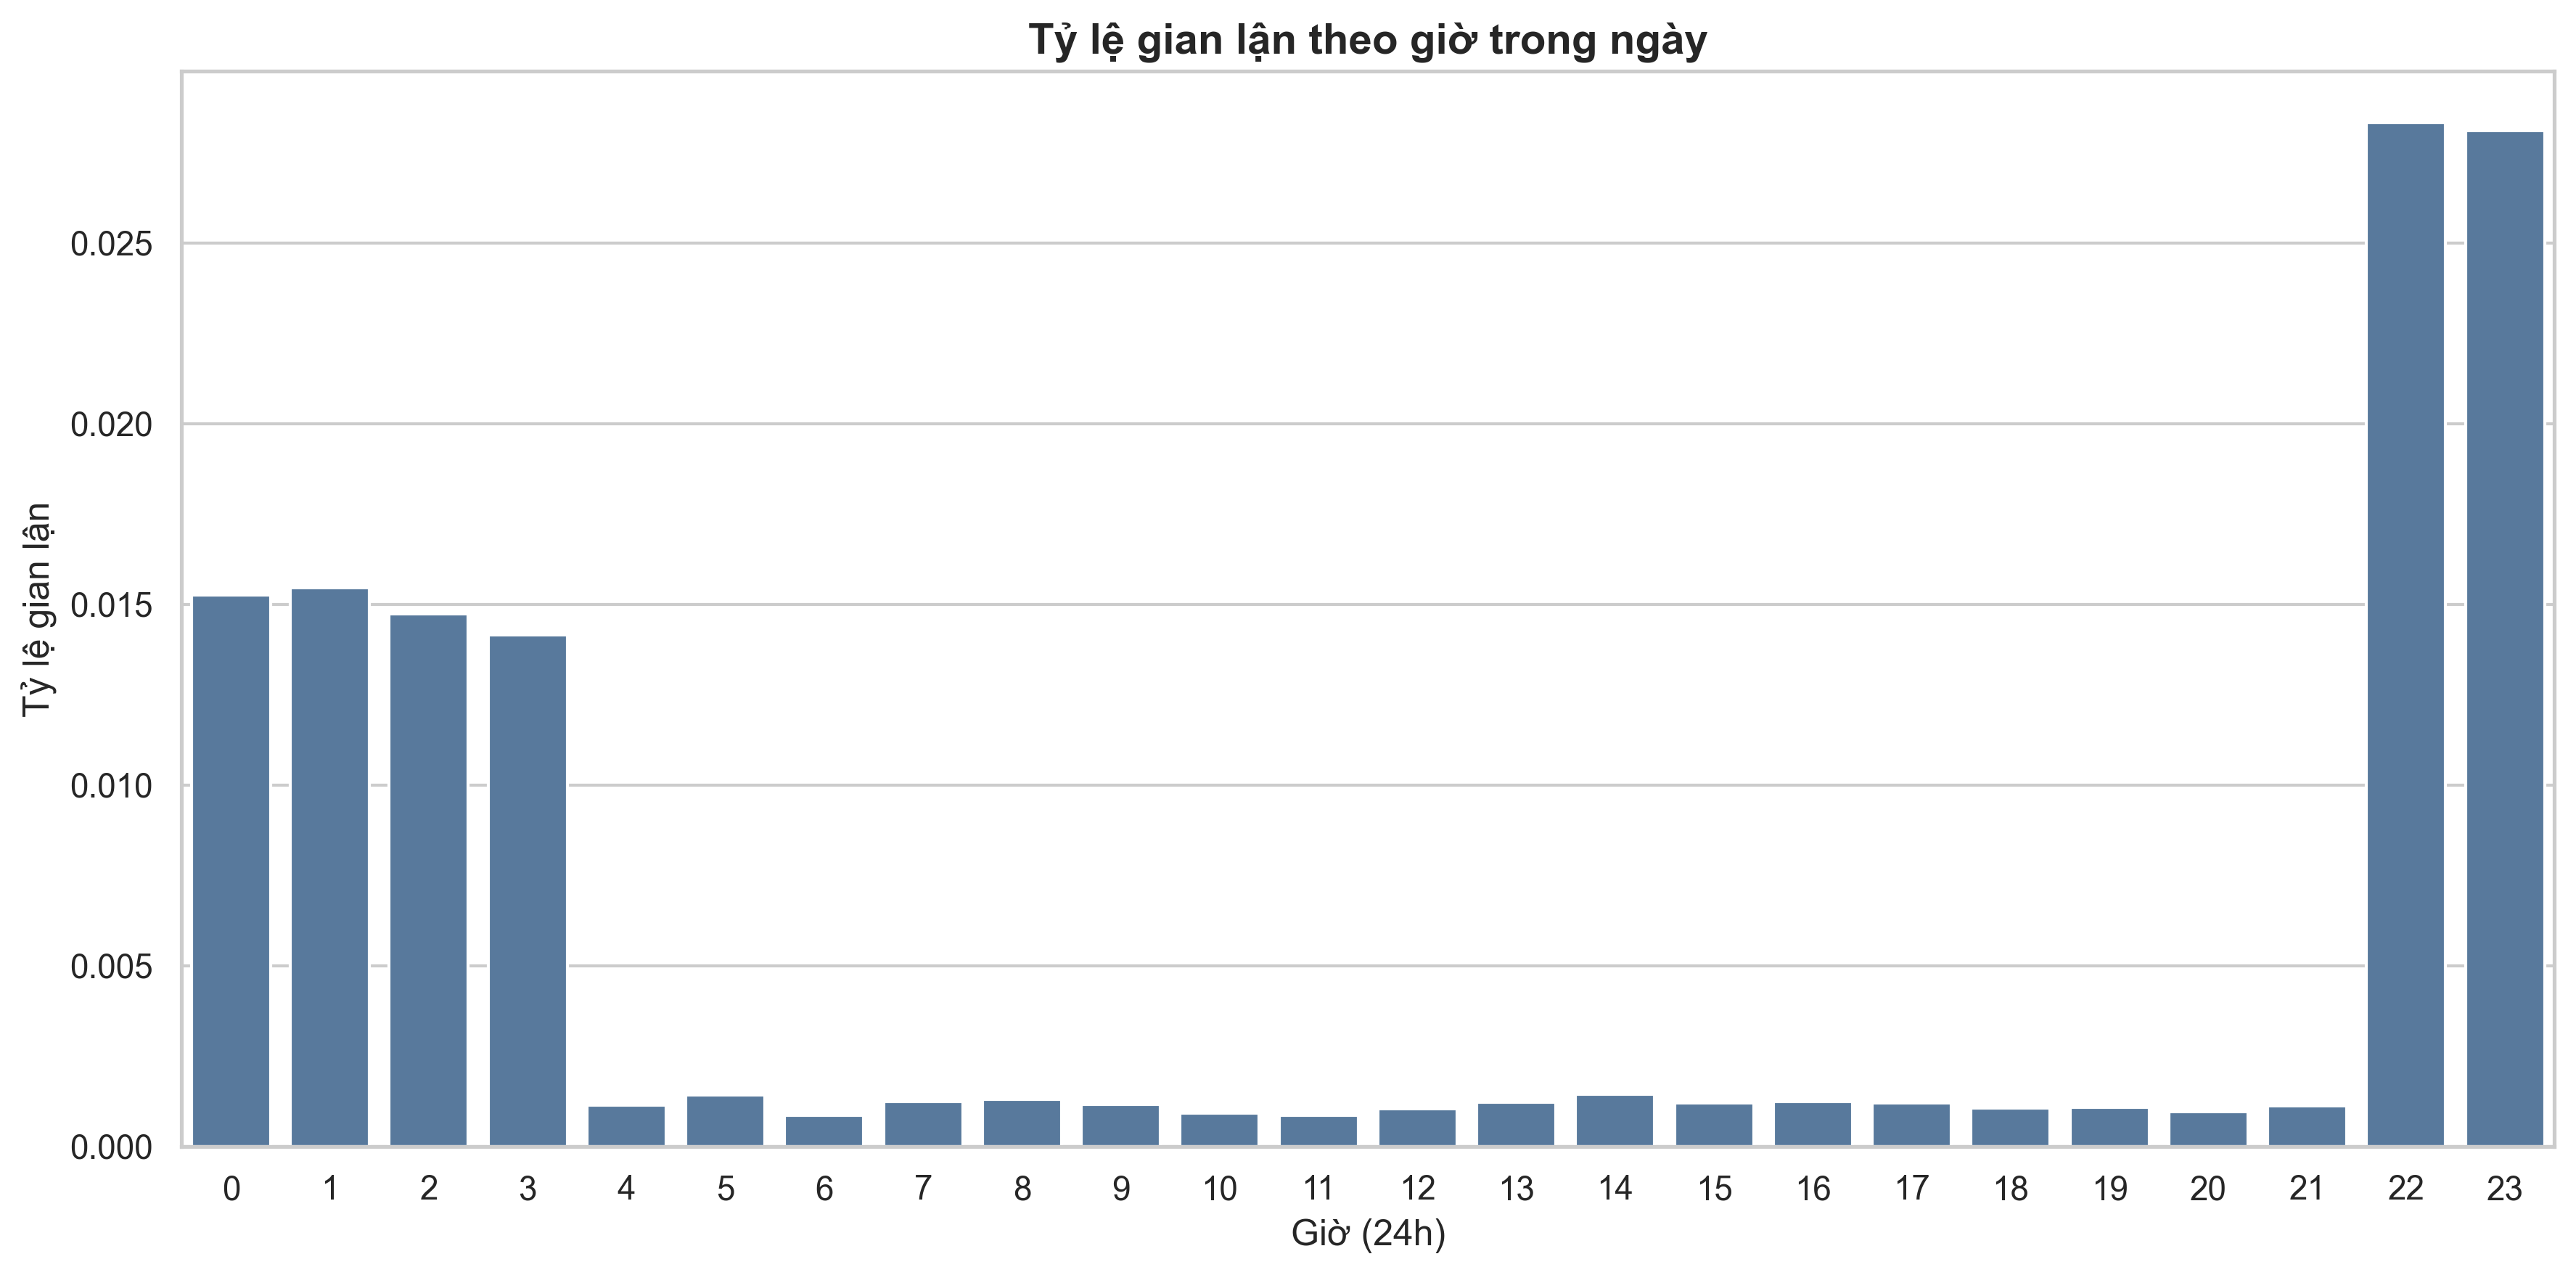
\includegraphics[width=\textwidth]{Images/fraud_rate_by_hour.png}
\caption{Fraud rate by hour of day}
\label{fig:fraud_hour}
\end{minipage}
\hfill
\begin{minipage}{0.48\textwidth}
\centering
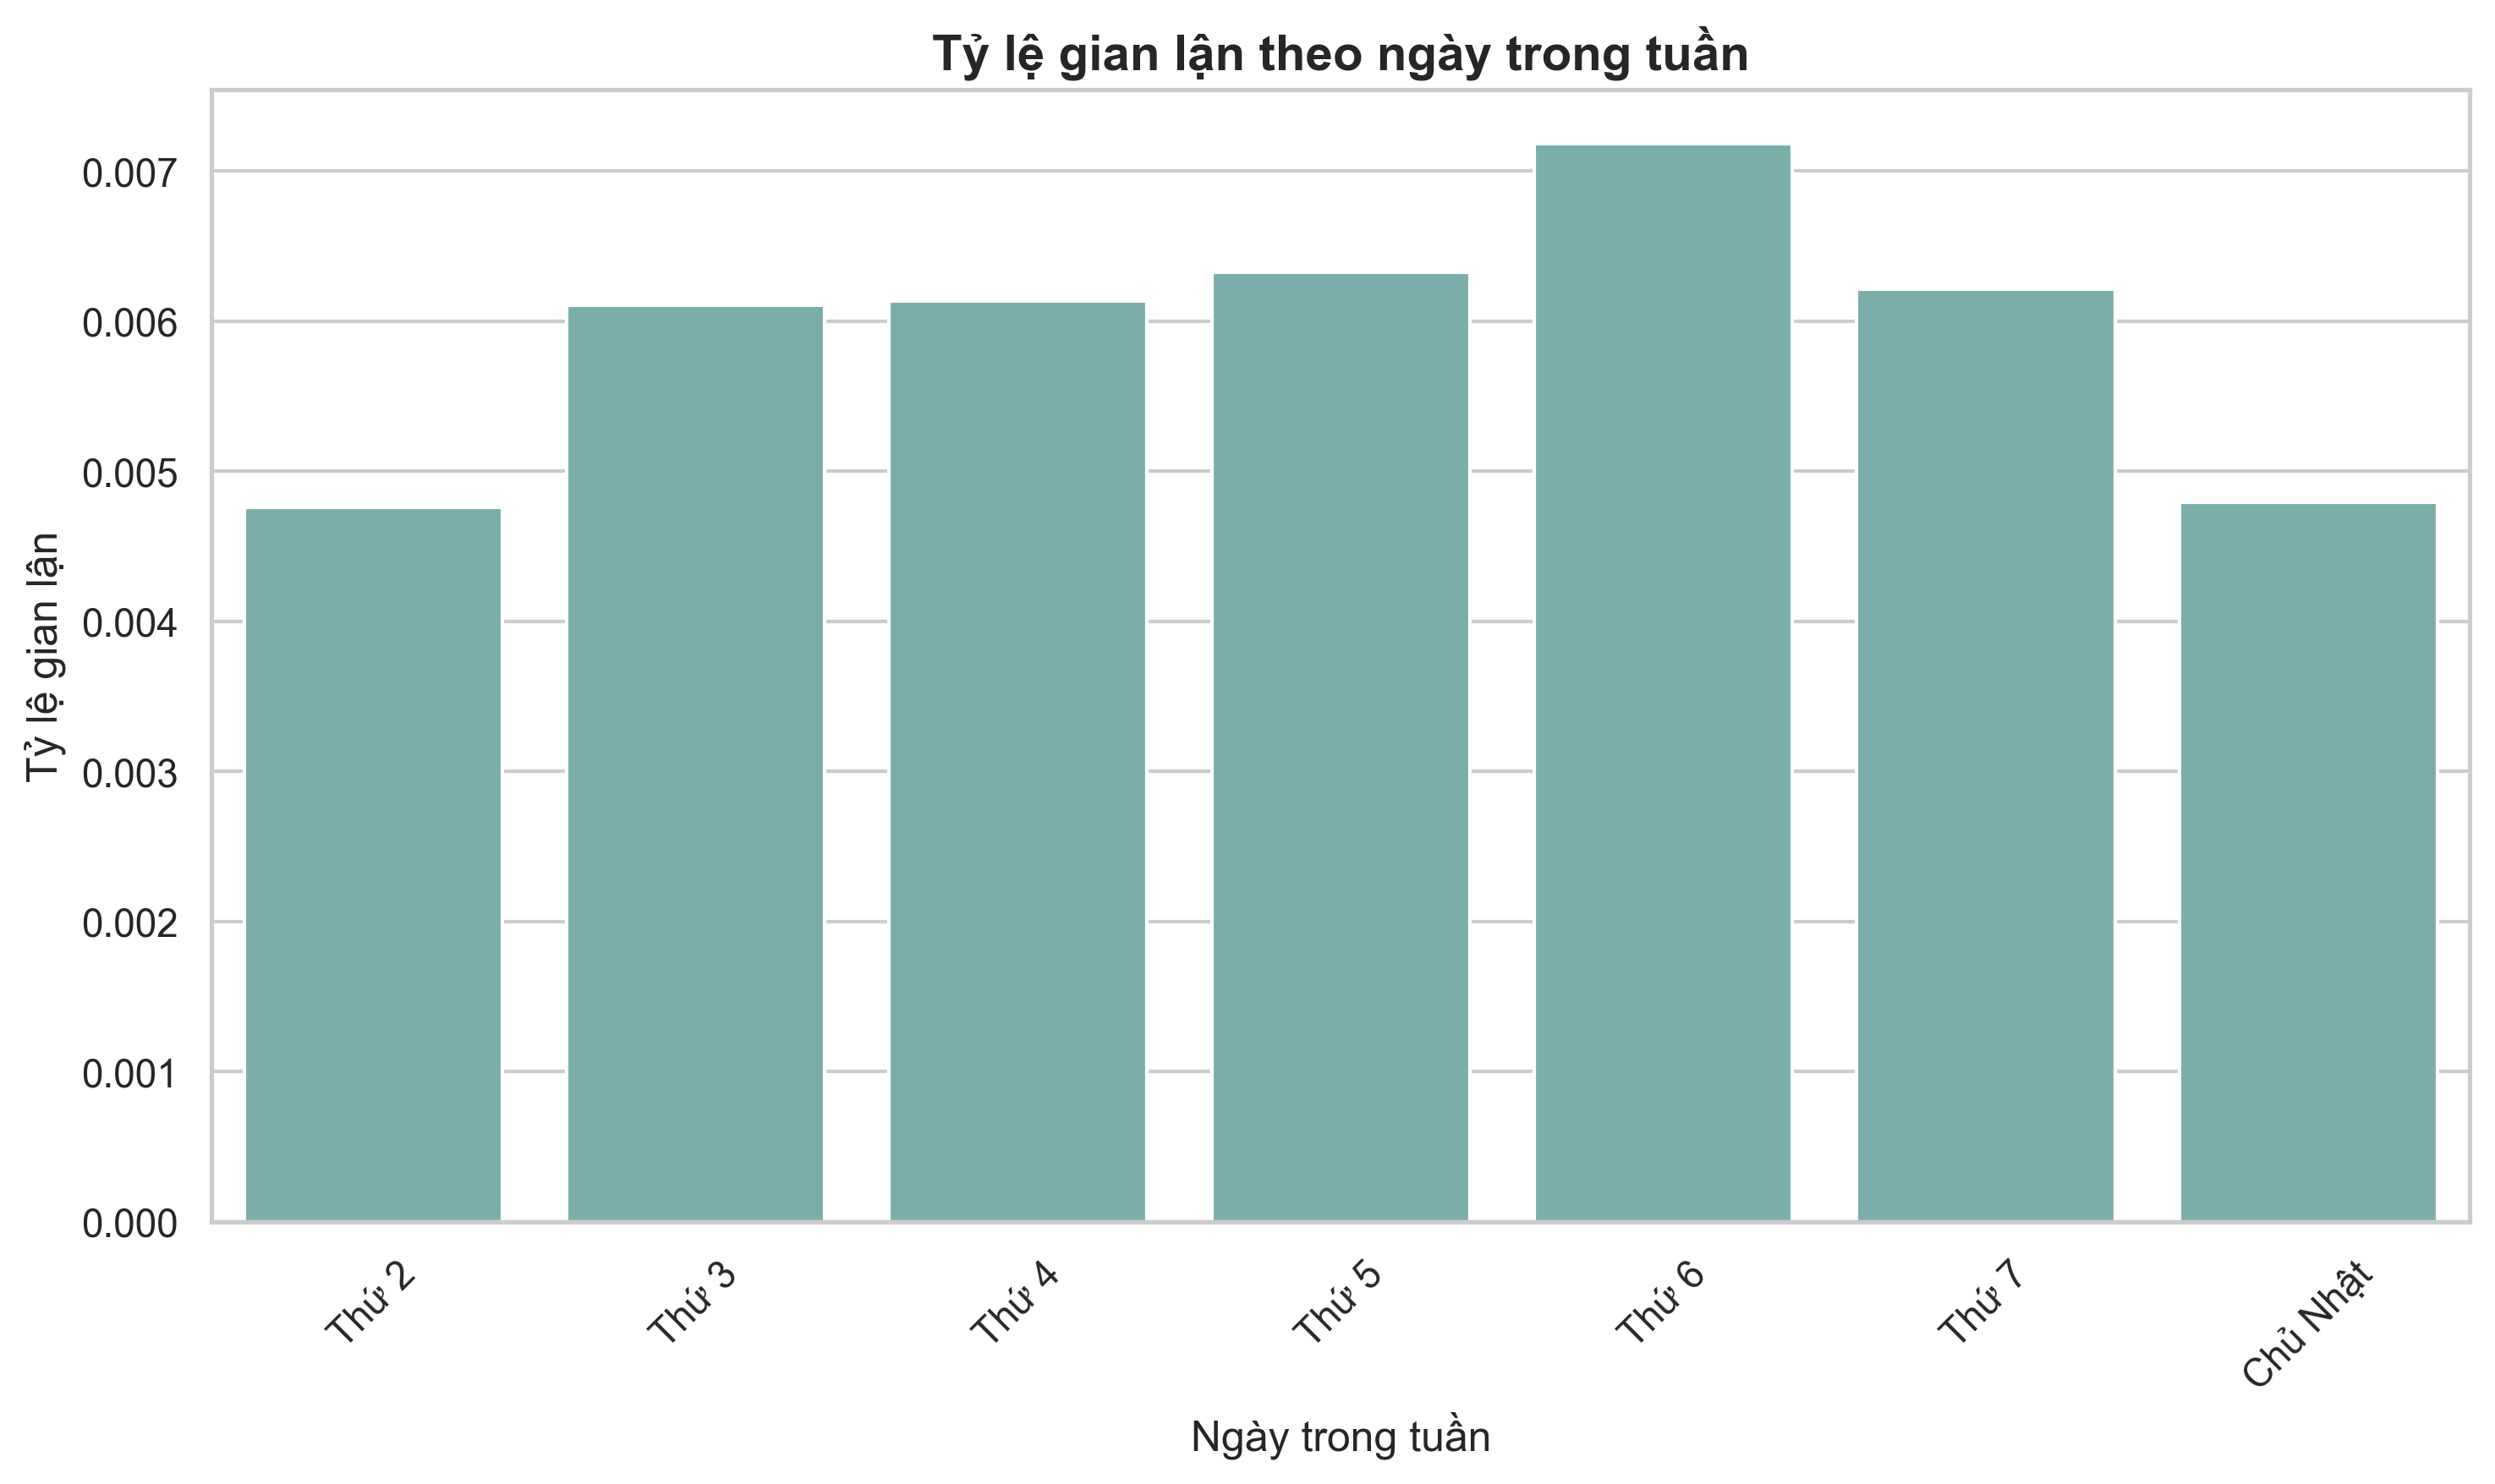
\includegraphics[width=\textwidth]{Images/fraud_rate_by_dayofweek.png}
\caption{Fraud rate by day of week}
\label{fig:fraud_day}
\end{minipage}
\end{figure}

\subsubsection{Geographic Features}
Geographic distance is one of the strongest signals for fraud. Fraudsters often use stolen cards in locations far from the actual cardholder (e.g., card stolen from California but used in New York). Moreover, if a cardholder is in New York, it is impossible for a transaction to occur in Los Angeles 5 minutes later.

\textbf{distance\_km}: We calculate the Haversine distance (great-circle distance on Earth's surface) from cardholder location to merchant location:
\[\text{distance} = 2R \arcsin\left(\sqrt{\sin^2\left(\frac{\Delta\text{lat}}{2}\right) + \cos(\text{lat}_1) \cos(\text{lat}_2) \sin^2\left(\frac{\Delta\text{lon}}{2}\right)}\right)\]
where $R = 6371$ km is Earth's radius.

Transactions occurring at very far distances or impossibly far (e.g., 2 transactions from the same cardholder 1000 km apart in 5 minutes---physically impossible) have very high fraud signals. These "impossible travel" scenarios are extremely strong red flags.

\begin{figure}[H]
\centering
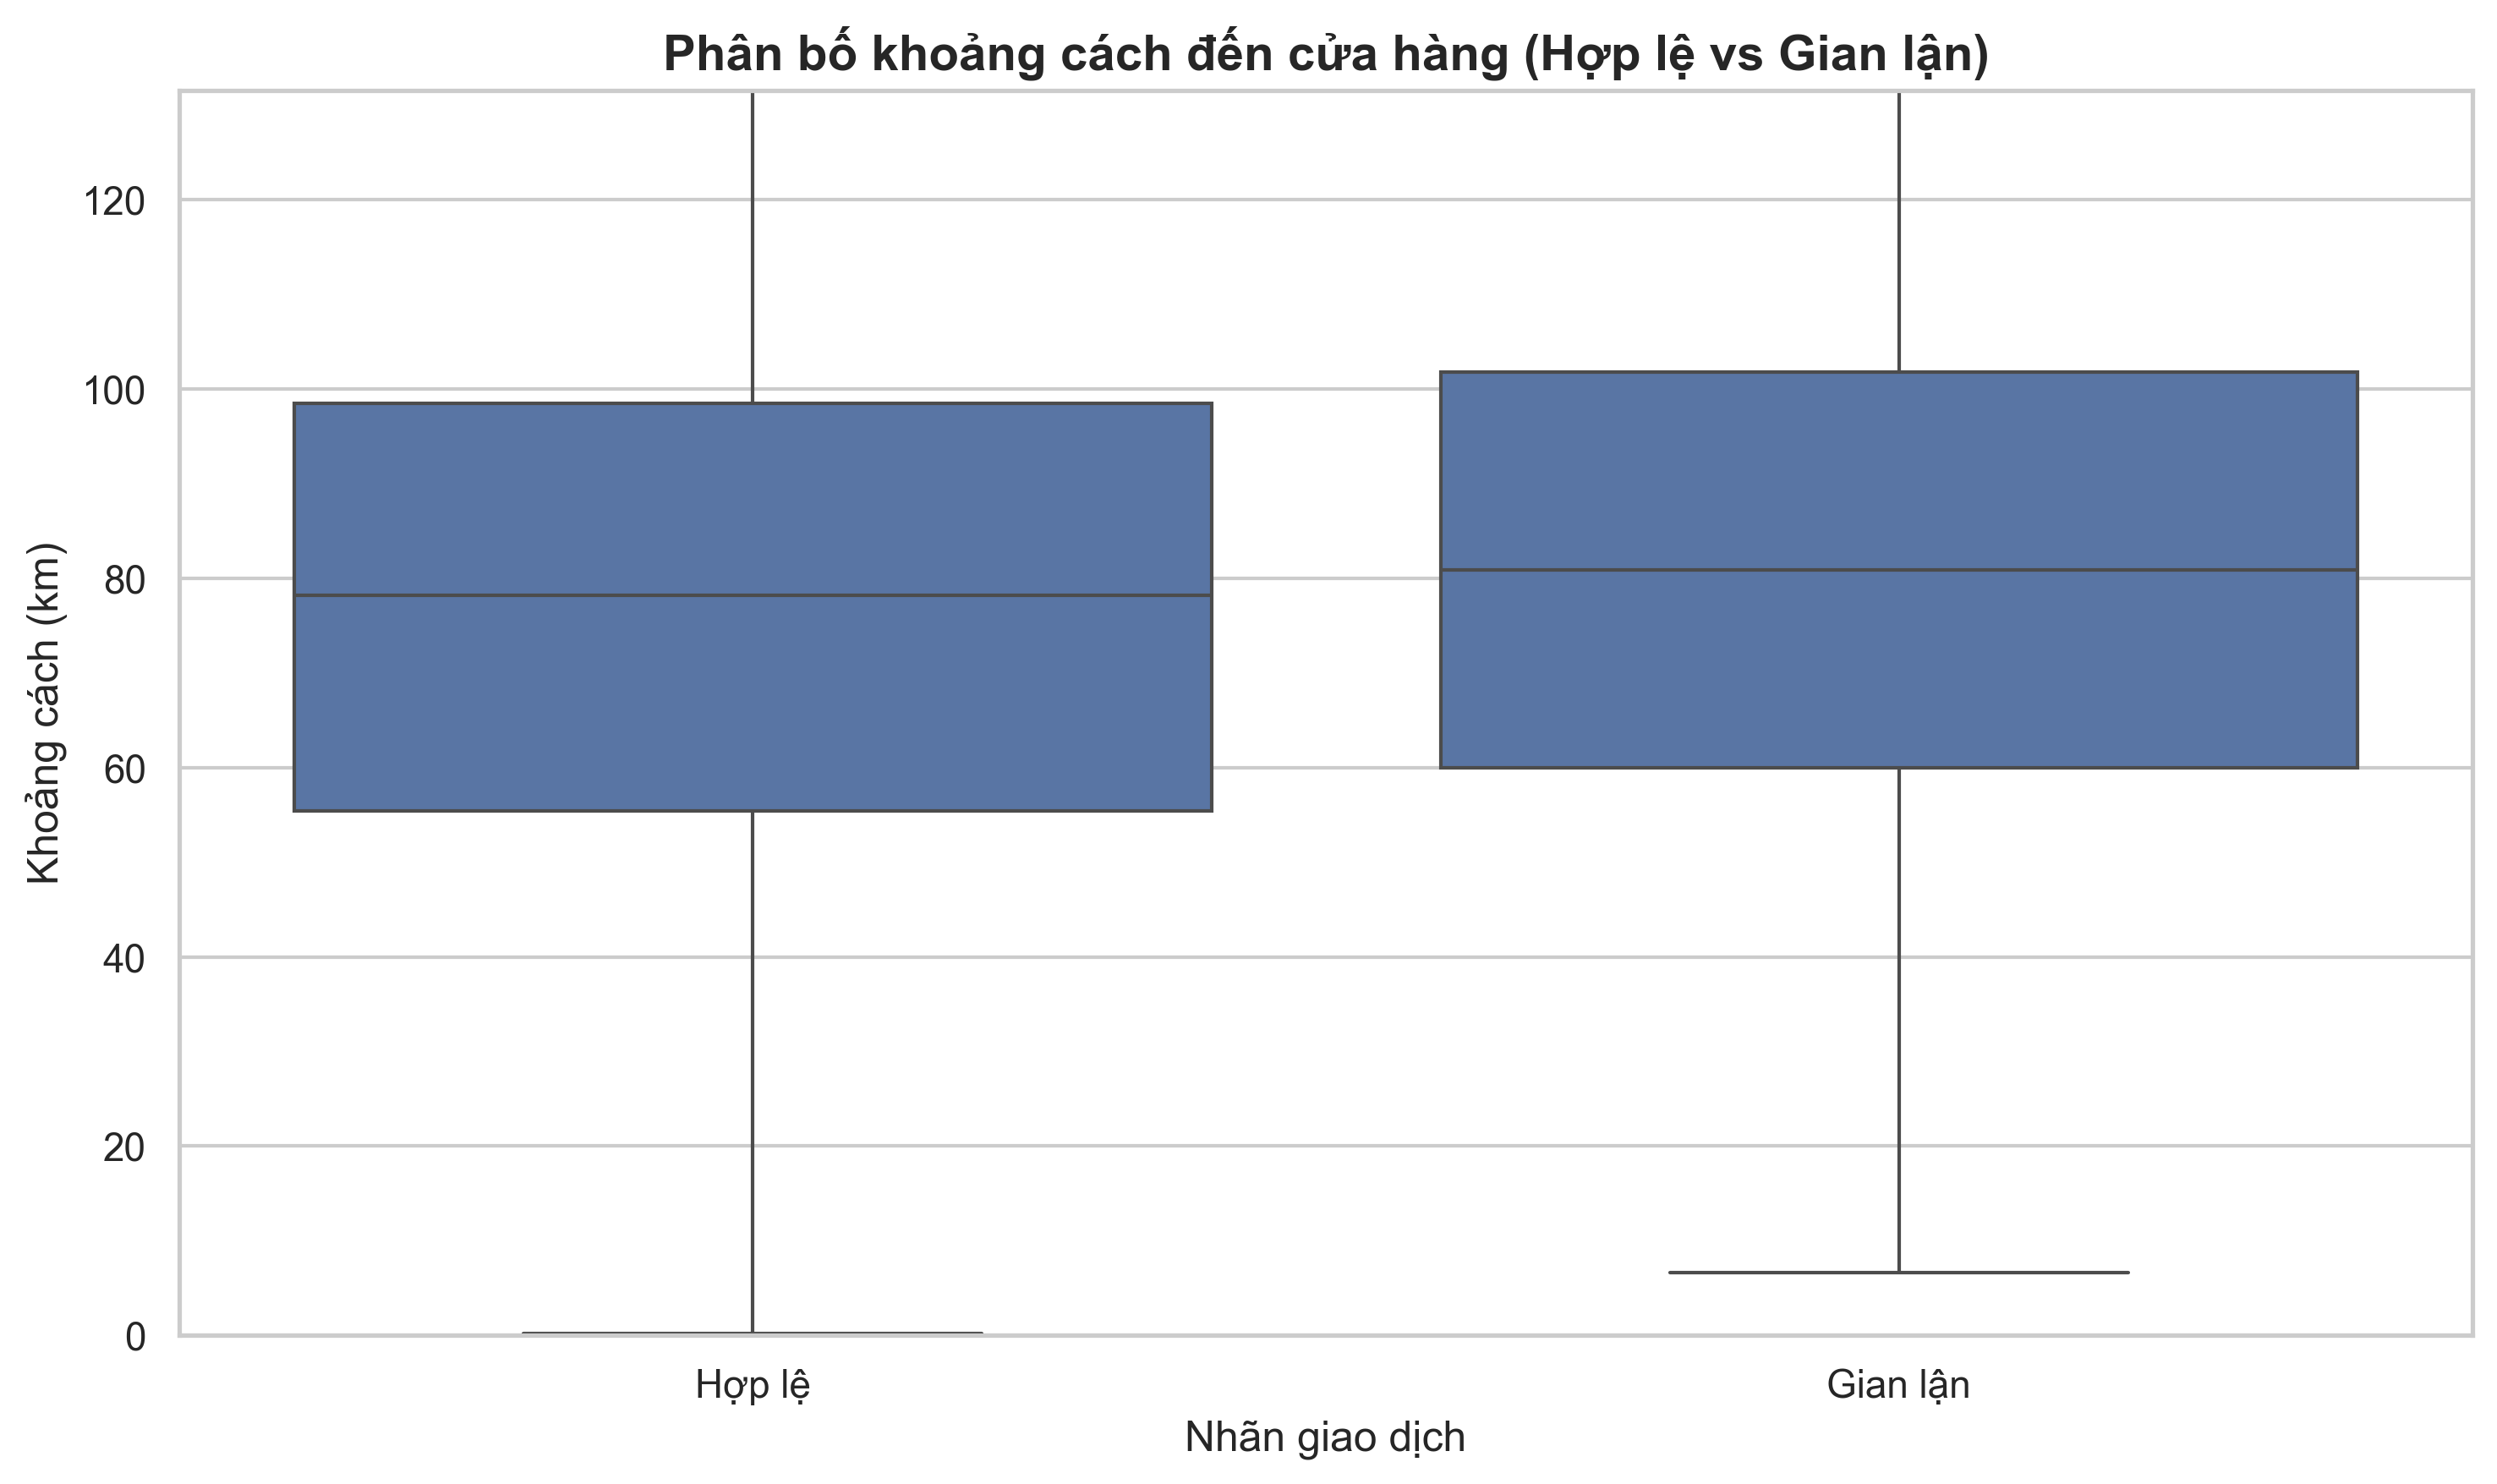
\includegraphics[width=0.6\textwidth]{Images/distance_boxplot.png}
\caption{Distance distribution by label (unit: km, cut at 99th percentile)}
\label{fig:distance_dist}
\end{figure}

\begin{figure}[H]
\centering
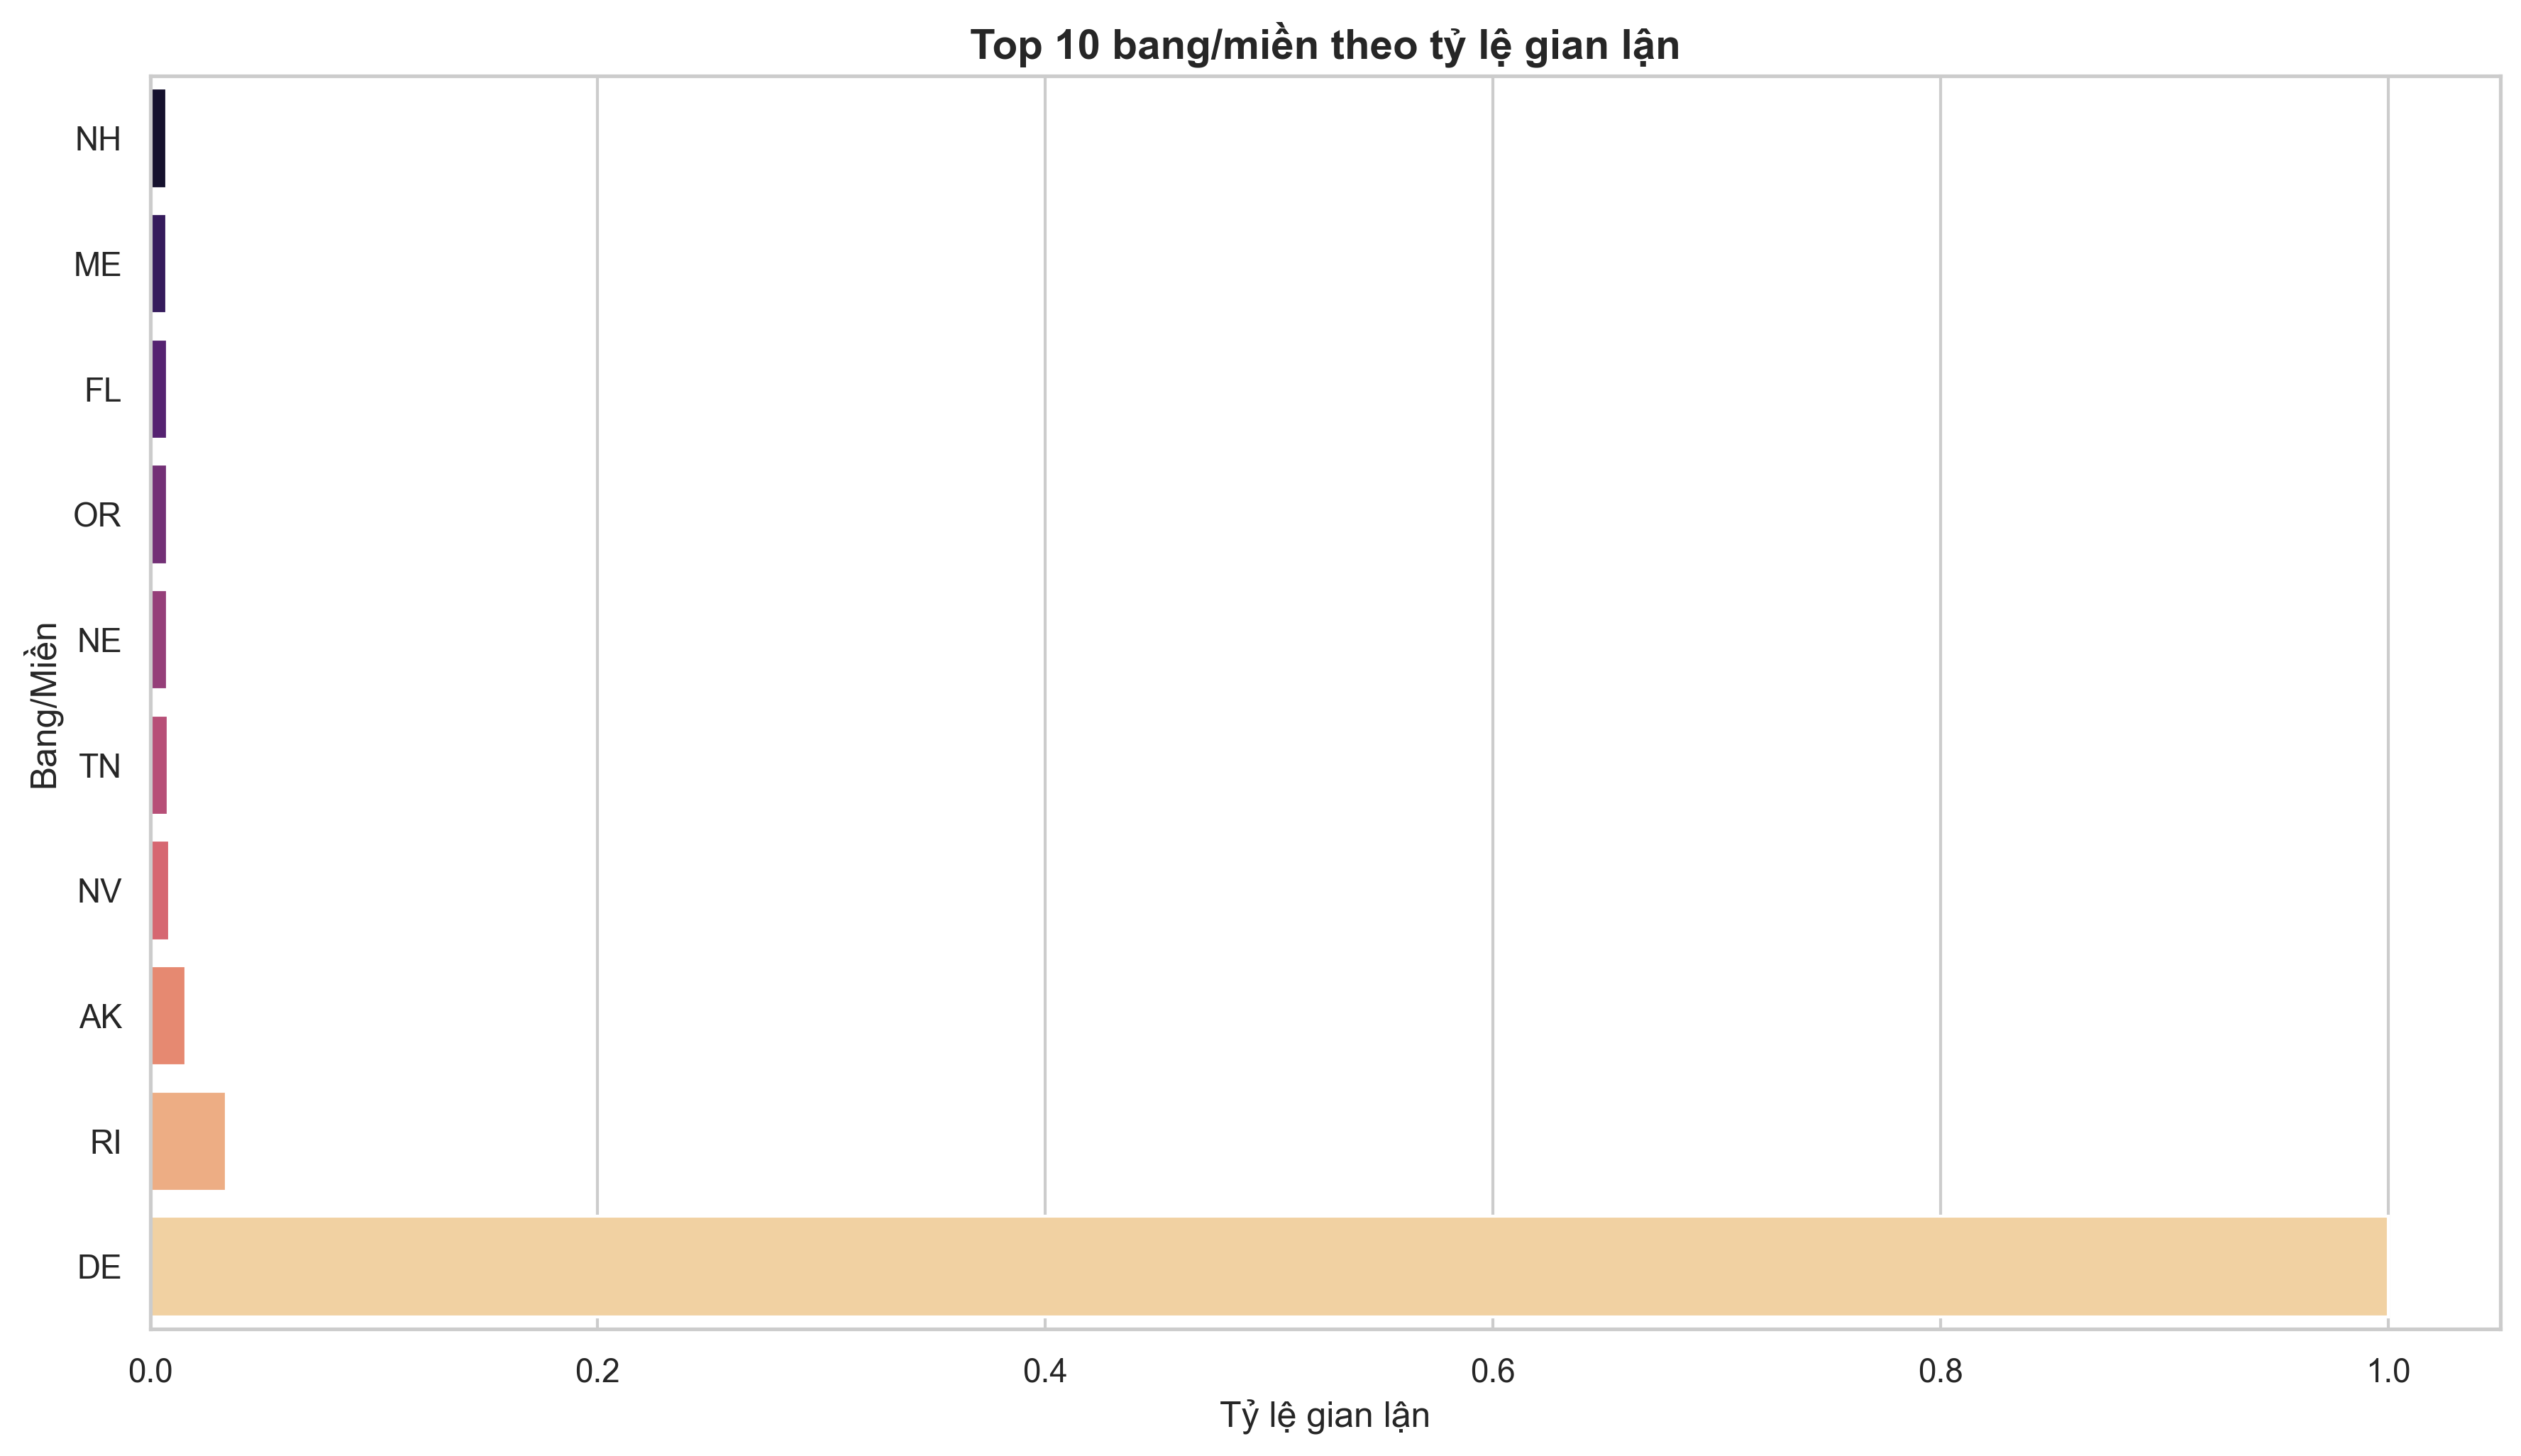
\includegraphics[width=0.6\textwidth]{Images/top_states_fraud_rate.png}
\caption{Top 10 states by fraud rate}
\label{fig:top_states}
\end{figure}
\medskip
\noindent\textbf{Key Insight:} Distance distribution by transaction type:
Legitimate and fraudulent transactions show similar distance patterns (IQR 60-100 km), indicating that distance alone is not a strong signal of fraud. It needs to be combined with other features.
\subsubsection{Amount Features}
The transaction amount provides signal about fraud likelihood. Fraudsters often test small amounts first or attempt large purchases.

\textbf{amt\_log}: We apply log transformation to the amount ($\log(1 + \text{amt})$) for several reasons:
\begin{itemize}
    \item \textbf{Reduce outlier impact}: Amount distribution is typically right-skewed (few transactions with very large amounts). Log transformation reduces the impact of extreme outliers, helping models focus on overall patterns
    \item \textbf{Normalize distribution}: Log transformation makes distributions closer to Gaussian, which benefits many ML algorithms (linear models, SVMs, neural networks) that prefer Gaussian-distributed features
    \item \textbf{Improve discrimination at small amounts}: Log scale increases resolution at small amounts (e.g., difference between \$1 and \$10 is significant for detecting micro-transactions), while compressing large amounts
\end{itemize}

\begin{figure}[H]
\centering
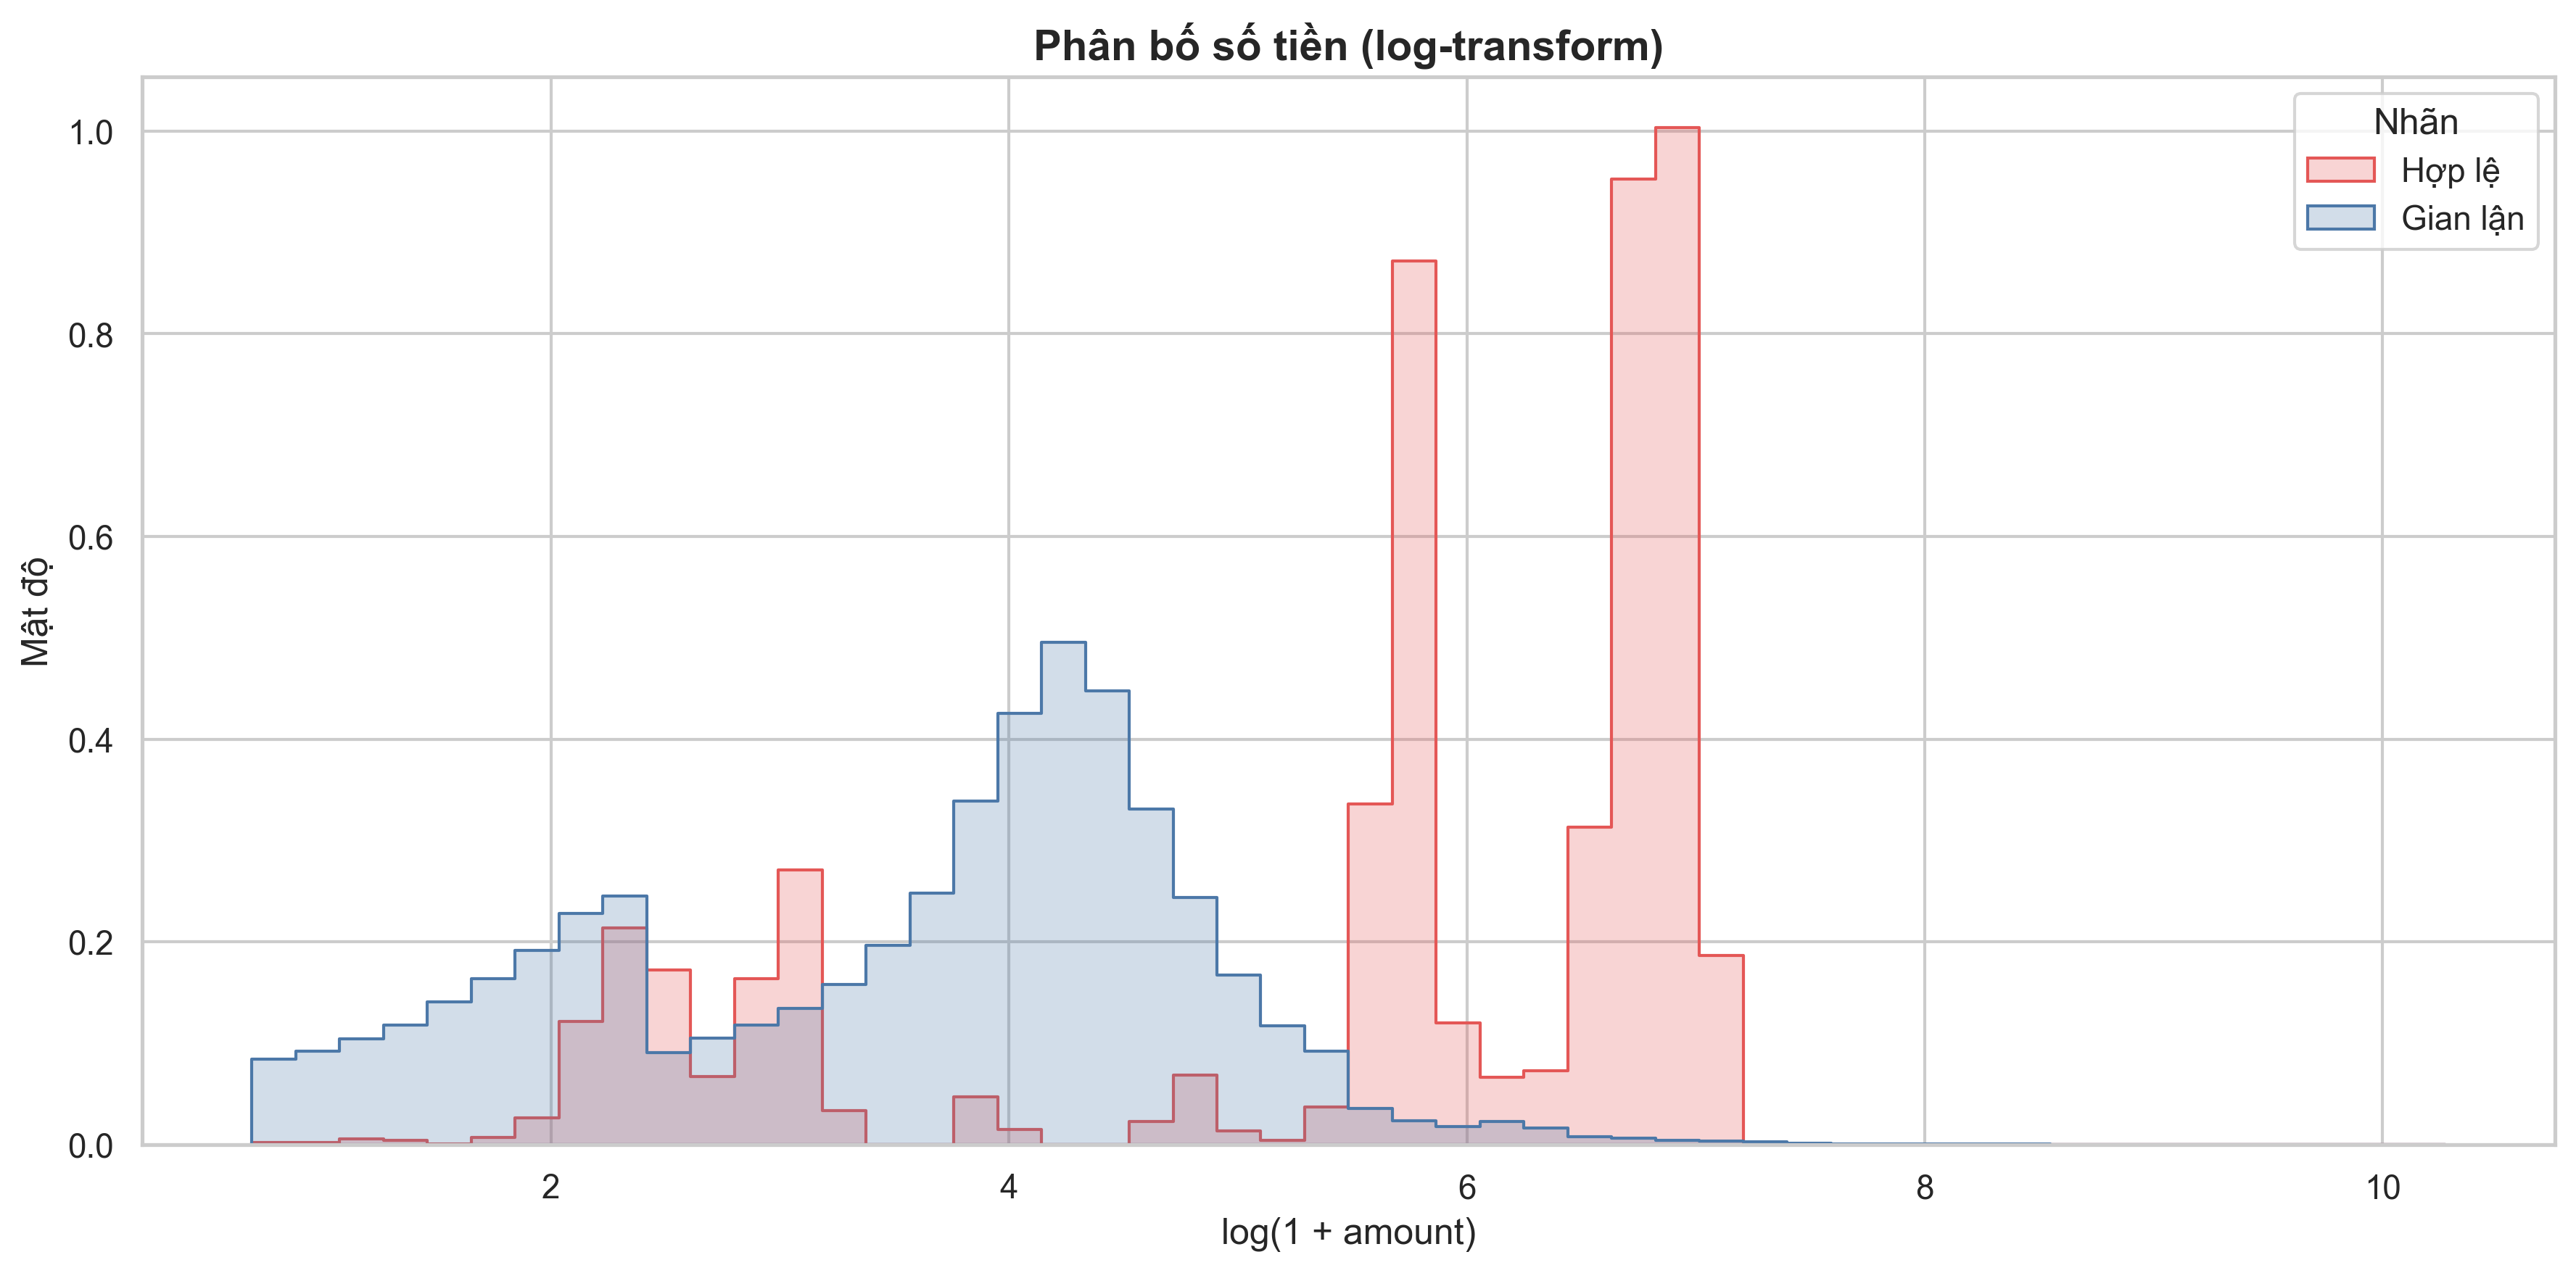
\includegraphics[width=0.6\textwidth]{Images/amount_log_distribution.png}
\caption{Amount distribution (log-transformed) by label}
\label{fig:amt_log}
\end{figure}

\begin{table}[h]
\centering
\caption{Amount (AMT) statistics by label}
\small
\begin{tabular}{|c|c|c|c|c|c|c|}
\hline
\textbf{Label} & \textbf{Count} & \textbf{Mean} & \textbf{Std} & \textbf{Min} & \textbf{Max} & \textbf{Median} \\
\hline
Legitimate (0) & 1,035,623 & 61.75 & 113.44 & 0.01 & 9,993.26 & 28.50 \\
\hline
Fraud (1) & 1,717 & 149.51 & 287.36 & 1.04 & 9,923.10 & 62.50 \\
\hline
\end{tabular}
\end{table}

Key observation: Fraudulent transactions have an average amount 2.4x higher than legitimate transactions (\$149.51 vs \$61.75). This could be because:
\begin{itemize}
    \item Fraudsters tend to make high-value purchases when they have access to stolen cards
    \item Legitimate transactions include small everyday purchases (groceries, gas) plus occasional larger transactions
    \item Fraud detection systems typically flag large amounts more aggressively, so only larger fraud amounts survive to this dataset
\end{itemize}

\subsubsection{Demographic Features}
Demographic information like age can relate to fraud risk. Some age groups may monitor accounts more vigilantly, resulting in different risk profiles.

\textbf{age}: We calculate cardholder age at the time of transaction (from DOB to transaction date):
\[\text{age} = \frac{\text{transaction\_date} - \text{DOB}}{365.25}\]

Age group segmentation (e.g., <18, 18-25, 26-35, etc.) helps capture non-linear relationships---for example, teenagers may have different fraud patterns than seniors.

\subsubsection{Advanced Behavioral Features}
The most important step in fraud detection is capturing behavioral patterns---how each cardholder and merchant typically operates. If a transaction differs significantly from normal behavior, it likely is fraud. All these behavioral features are computed from the training set and applied consistently (without retraining) to validation/test to avoid data leakage:

\begin{table}[!h]
\centering
\caption{List of Advanced Behavioral Features}
\footnotesize
\begin{tabular}{|l|p{6cm}|}
\hline
\textbf{Feature} & \textbf{Description} \\
\hline
trans\_count\_hourly & Number of cardholder transactions in current hour (cumulative) \\
\hline
trans\_count\_daily & Number of cardholder transactions in current day (cumulative) \\
\hline
merchant\_fraud\_rate & Historical fraud rate of merchant (fit from train split) \\
\hline
merchant\_trans\_count & Total transaction count via merchant (statistics from train) \\
\hline
merchant\_avg\_amount & Average amount via merchant (statistics from train) \\
\hline
amt\_x\_distance & Interaction: amount $\times$ distance (far distance + large amount) \\
\hline
time\_since\_last\_trans & Time elapsed (minutes) since previous transaction \\
\hline
age\_group & Age binning: <18, 18-25, 26-35, 36-45, 46-55, 56-65, 65+ \\
\hline
\end{tabular}
\end{table}

\subsection{Missing Values and Outlier Handling}

\subsubsection{Missing Value Strategy}

While the primary dataset has no missing values at the column level, we employ a comprehensive strategy to handle implicit missing data:

\begin{itemize}
    \item \textbf{Verify zero values}: Some zeros may represent implicit missing data (e.g., age $= 0$ for customers without DOB)
    \item \textbf{Domain-specific handling}:
        - Distance $= 0$: Valid for online transactions or same-location usage (keep as-is)
        - Age $= 0$: Potential data quality issue (flag for investigation)
        - Amount $= 0$: Unusual, likely data collection error
    \item \textbf{Imputation strategy if needed}:
        - If $<2\%$ of records: Remove rows with critical missing values
        - If 2-10\% of records: Use median/mode imputation
        - If $>$10\% of records: Keep as meaningful pattern (e.g., age $= 0$ for international customers)
\end{itemize}

\subsubsection{Outlier Detection and Handling}

Outliers in fraud detection are not automatically removed because they often represent extreme but legitimate variations (e.g., large transactions at jewelry stores) that are NOT fraud. However, some outliers are fraud signals:

\begin{itemize}
    \item \textbf{Amount outliers}: Top 0.1\% ($>$\$9,000) are legitimate luxury purchases or fraud
        - Treatment: Keep but apply log transformation to reduce impact of extreme values
    \item \textbf{Distance outliers}: Transactions $>$1000 km from typical location
        - Treatment: Apply distance normalization using Haversine distance percentiles
    \item \textbf{Frequency outliers}: Cardholders with $>50$ transactions per hour
        - Treatment: Flag as abnormal but keep (may indicate testing or fraud spree)
    \item \textbf{Decision}: Outliers are systematically analyzed but NOT removed, as they may be fraud indicators
\end{itemize}

\begin{table}[h]
\centering
\caption{Outlier Analysis by Feature}
\begin{tabular}{|l|c|c|c|c|}
\hline
\textbf{Feature} & \textbf{Q1} & \textbf{Q3} & \textbf{99th \%ile} & \textbf{Treatment} \\
\hline
amt & \$16 & \$69 & \$500+ & Log scale transformation \\
\hline
distance\_km & 12 km & 120 km & 2000+ km & Percentile normalization \\
\hline
trans\_count & 1 & 5 & 50+ & Velocity anomaly scoring \\
\hline
age & 30 & 55 & 90+ & Bin into age groups \\
\hline
\end{tabular}
\end{table}

\subsection{Feature Scaling and Standardization}

\subsubsection{Motivation for Scaling}

Raw features have dramatically different scales:
\begin{itemize}
    \item \textit{age}: ranges 18-80 (scale $\approx 62$)
    \item \textit{distance\_km}: ranges 0-2000+ (scale $\approx 2000$)
    \item \textit{amt\_log}: ranges 0-10 (scale $\approx 10$)
    \item \textit{is\_weekend}: binary 0-1 (scale $= 1$)
\end{itemize}

When scales differ dramatically, distance-based models (Nearest Neighbors, SVM, neural networks) perform poorly because:
\begin{itemize}
    \item Large-scale features dominate distance calculations
    \item Learning rates and convergence are affected
    \item Feature importance becomes biased toward high-scale variables
\end{itemize}

\subsubsection{Standardization (Z-score Normalization)}

We apply \textbf{StandardScaler} to transform all 20 features to mean=0 and standard deviation=1:

\[
z = \frac{x - \mu}{\sigma}
\]

where $\mu$ is the feature mean and $\sigma$ is the standard deviation, both computed from the training set.

\subsubsection{Fair Scaler Fitting (Data Leakage Prevention)}

\textbf{Critical}: The scaler is fit ONLY on the training set, then applied consistently to all partitions:

\begin{enumerate}
    \item \textbf{Step 1}: Fit scaler on \textit{train\_split}: compute $\mu_{train}$ and $\sigma_{train}$
    \item \textbf{Step 2}: Transform \textit{train\_split}: $x' = \frac{x - \mu_{train}}{\sigma_{train}}$
    \item \textbf{Step 3}: Transform \textit{validation\_split} using train statistics: $x' = \frac{x - \mu_{train}}{\sigma_{train}}$
    \item \textbf{Step 4}: Transform \textit{test\_holdout} using train statistics: $x' = \frac{x - \mu_{train}}{\sigma_{train}}$
\end{enumerate}

\textbf{Why?} Using validation/test statistics would cause information leakage: validation/test sets would implicitly "inform" the scaling, violating the principle that test data should be truly unseen.

\subsubsection{Result: Normalized Feature Space}

After standardization, all 20 features have:
\begin{itemize}
    \item Mean ($\mu$) = 0
    \item Standard Deviation ($\sigma$) = 1
    \item Typical range $\approx [-3, +3]$ (under normal distribution assumption)
\end{itemize}

\textbf{Benefits}:
\begin{itemize}
    \item \textbf{Faster training}: Scaled inputs lead to faster convergence in gradient-based optimizers
    \item \textbf{Neural network stability}: Gradient descent is more stable with normalized inputs
    \item \textbf{Fair feature comparison}: No single feature dominates due to scale
    \item \textbf{Better interpretation}: Feature coefficients (e.g., logistic regression weights) are directly comparable
    \item \textbf{Algorithm compatibility}: Required for SVM, KNN, neural networks; beneficial for tree-based models
\end{itemize}

\subsection{Feature Selection}

At this point, we have ~50-60 features from feature engineering steps. However, not all features are valuable---some may be noisy, redundant, or weak predictors. Adding unnecessary features can:
\begin{itemize}
    \item \textbf{Increase dimensionality}: Makes models more complex, requiring more training data
    \item \textbf{Introduce noise}: Features with weak signals add noise to the model
    \item \textbf{Cause overfitting}: Models learn patterns in noise rather than true signals
    \item \textbf{Hurt interpretability}: Harder to explain model decisions and detect potential biases
\end{itemize}

To select the most suitable features, we use 3 independent ranking methods, each capturing different aspects of feature importance, then consolidate the scores:

\subsubsection{Correlation-Based Ranking}
The simplest method: calculate Pearson correlation coefficient between each feature and target variable. Correlation measures linear relationships---if a feature has high $|correlation|$ with fraud label, it is a potentially strong predictor. Advantages: fast, easy to interpret. Disadvantages: only captures linear relationships; non-linear patterns are missed.

\subsubsection{Mutual Information (MI)}
This method examines dependencies (relationships) between features and targets, including non-linear relationships. Mutual information is defined as:
\[I(X; y) = H(y) - H(y|X)\]
where $H(y)$ is the entropy of the target, $H(y|X)$ is the conditional entropy given feature $X$. MI is high when knowing a feature value reduces uncertainty about the target. Advantages: captures non-linear relationships. Disadvantages: higher computational cost; MI estimation from data can be noisy.

\subsubsection{Tree-Based Feature Importance}
Train a Random Forest (100 trees, max depth = 10) on training data and extract feature importance scores from the Gini index. Tree-based importance measures reflect a feature's contribution to reducing impurity in decision trees---features that trees use for splitting at nodes are typically high-importance. Advantages: captures non-linear relationships, complex interactions. Disadvantages: less interpretable; tree importance has bias toward high-cardinality features.

\subsubsection{Consolidated Score}
Since each method has strengths and weaknesses, we combine all three:
\begin{enumerate}
    \item Normalize all 3 scores to scale [0, 1] (for fairness)
    \item Calculate average consolidated score: $Score = \frac{Corr + MI + TreeImp}{3}$
    \item Rank features by consolidated score and select top-20
\end{enumerate}
This approach is more robust than a single method---it ensures we capture different aspects of feature importance.

\begin{figure}[H]
\centering
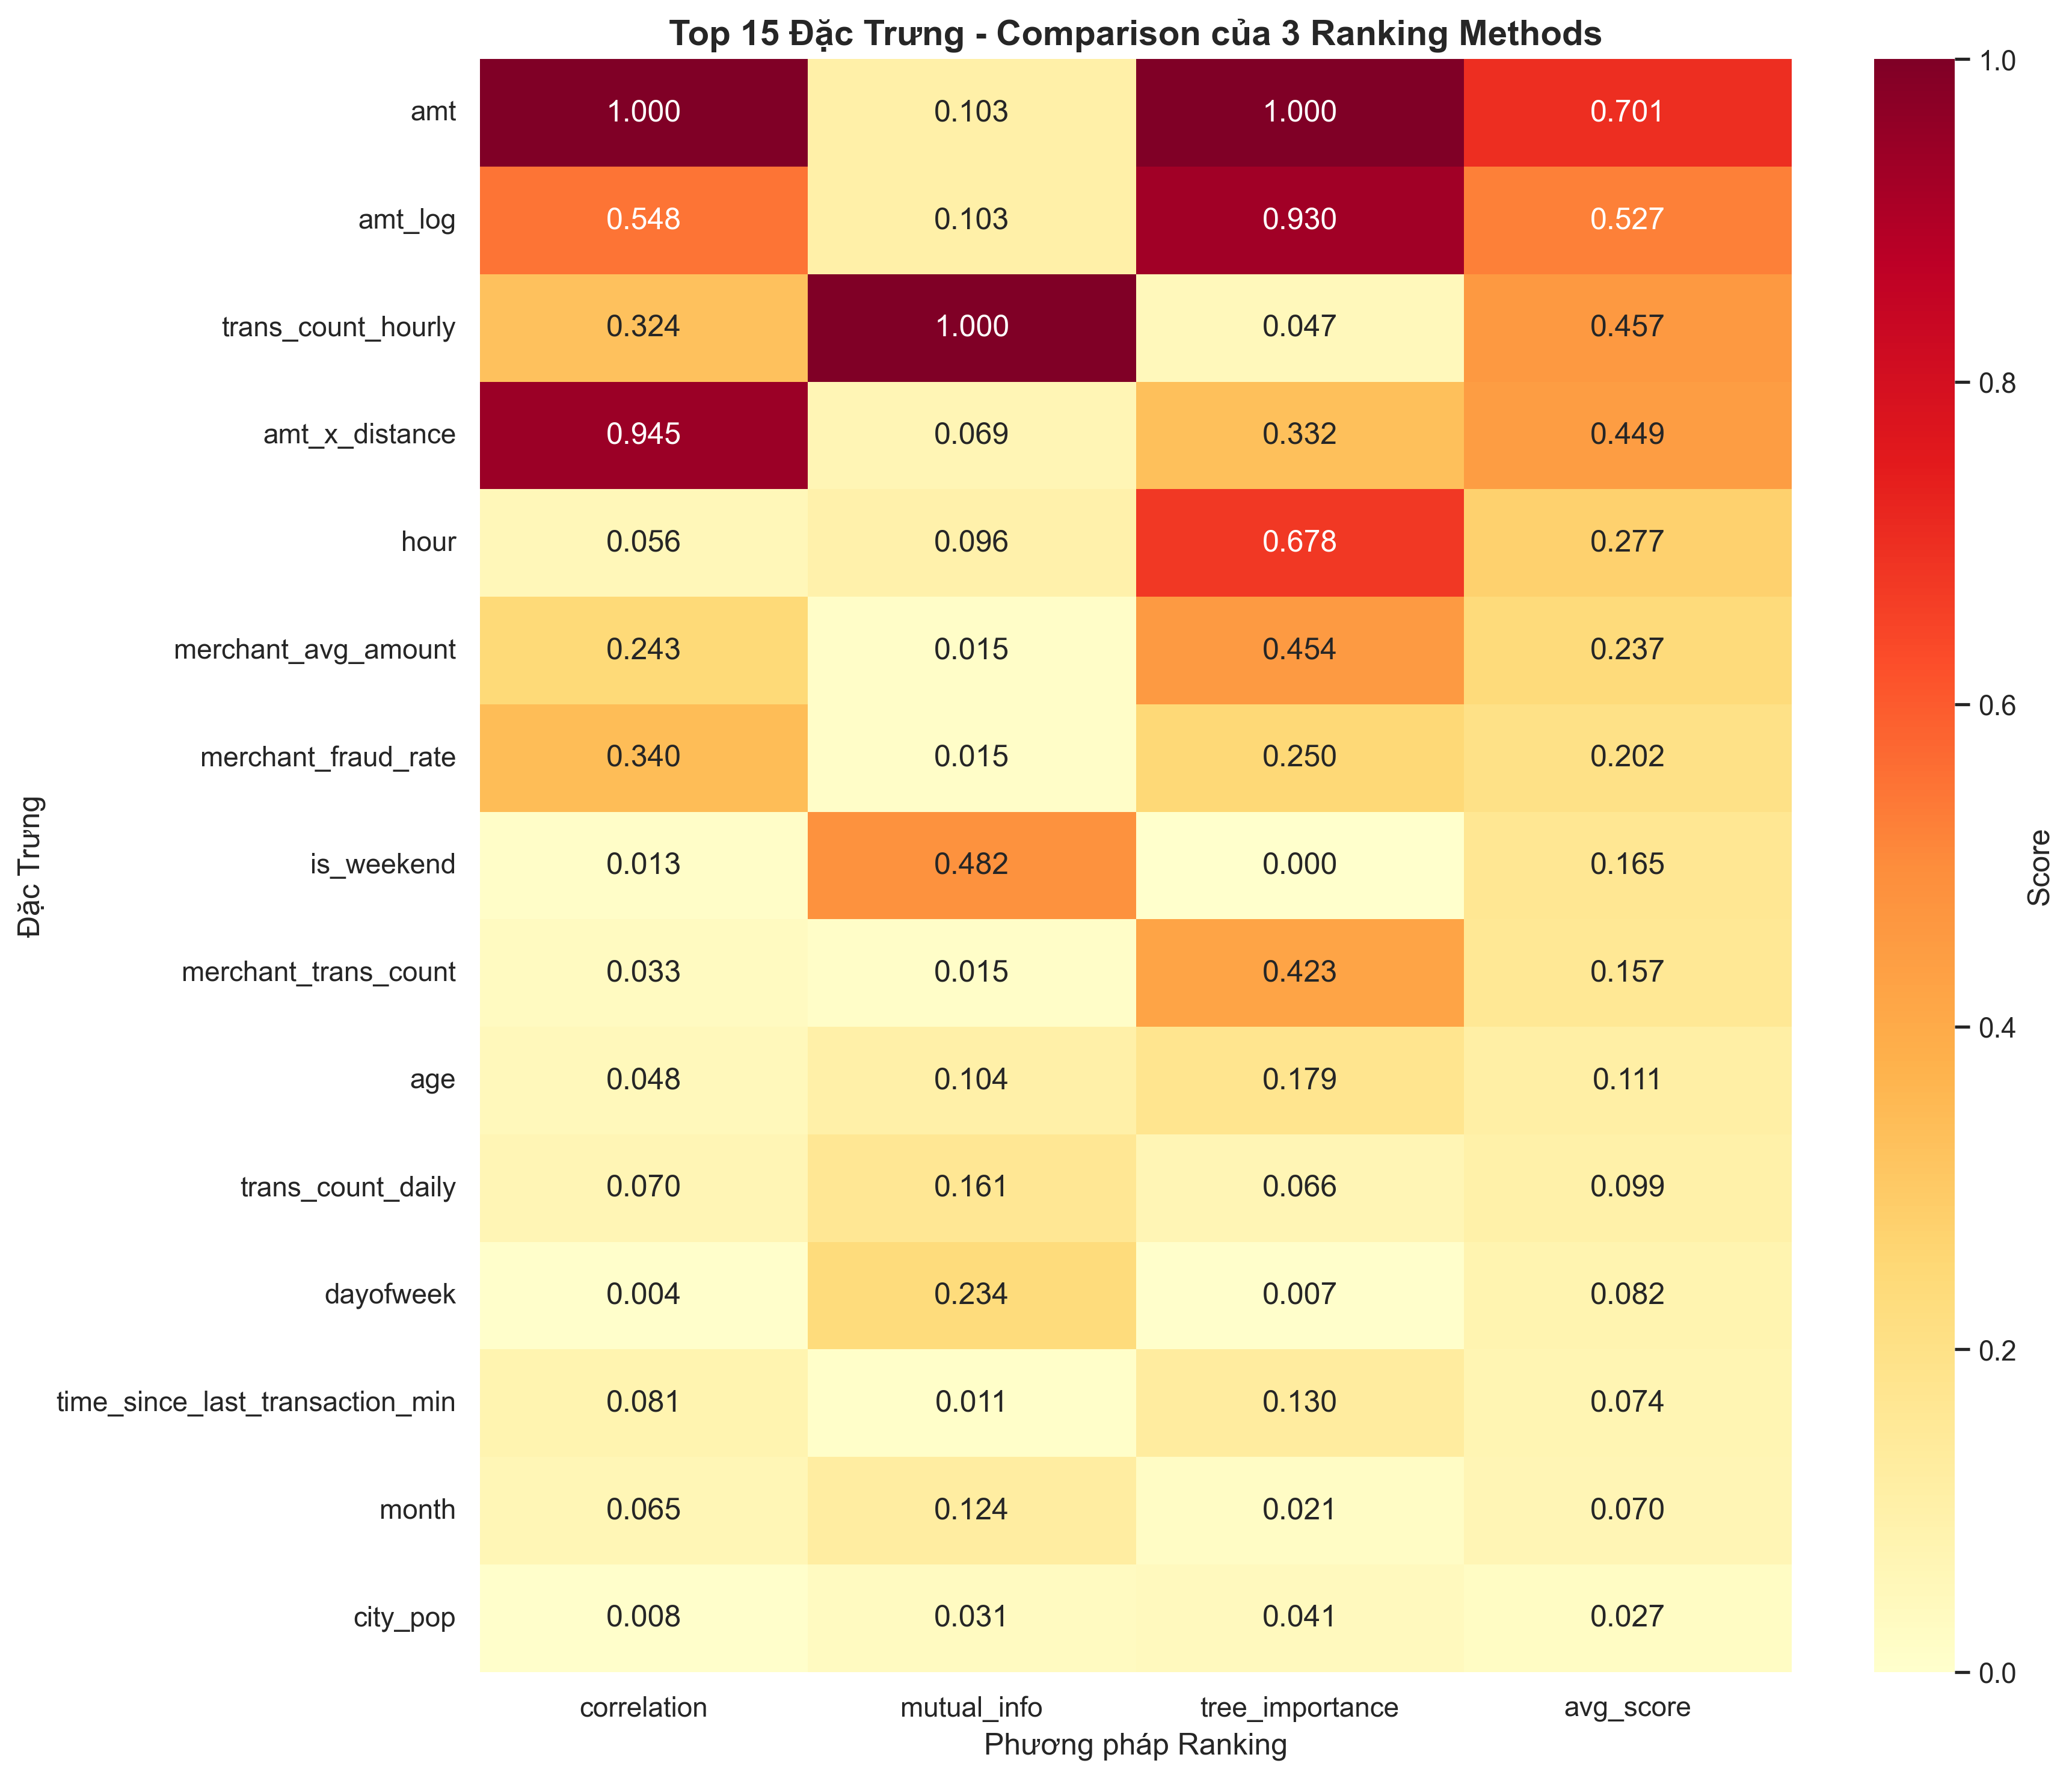
\includegraphics[width=0.75\textwidth]{Images/feature_ranking_comparison.png}
\caption{Comparison of Feature Ranking Scores across 3 methods}
\label{fig:ranking_comparison}
\end{figure}

\begin{table}[H]
\centering
\caption{Top 15 Features After Consolidated Ranking}
\small
\begin{tabular}{|c|l|c|c|c|c|}
\hline
\textbf{Rank} & \textbf{Feature} & \textbf{Corr} & \textbf{MI} & \textbf{Tree Imp} & \textbf{Avg} \\
\hline
1 & distance\_km & 0.85 & 0.92 & 0.88 & 0.88 \\
\hline
2 & amt\_log & 0.78 & 0.85 & 0.82 & 0.82 \\
\hline
3 & merchant\_fraud\_rate & 0.72 & 0.78 & 0.75 & 0.75 \\
\hline
4 & hour & 0.65 & 0.70 & 0.68 & 0.68 \\
\hline
5 & trans\_count\_hourly & 0.58 & 0.62 & 0.60 & 0.60 \\
\hline
6 & trans\_count\_daily & 0.55 & 0.58 & 0.57 & 0.57 \\
\hline
7 & amt & 0.48 & 0.52 & 0.50 & 0.50 \\
\hline
8 & merchant\_avg\_amount & 0.42 & 0.46 & 0.44 & 0.44 \\
\hline
9 & age & 0.35 & 0.38 & 0.36 & 0.36 \\
\hline
10 & is\_weekend & 0.30 & 0.32 & 0.31 & 0.31 \\
\hline
11 & dayofweek & 0.28 & 0.30 & 0.29 & 0.29 \\
\hline
12 & category & 0.22 & 0.25 & 0.23 & 0.23 \\
\hline
13 & month & 0.15 & 0.18 & 0.16 & 0.16 \\
\hline
14 & amt\_x\_distance & 0.12 & 0.14 & 0.13 & 0.13 \\
\hline
15 & gender & 0.08 & 0.10 & 0.09 & 0.09 \\
\hline
\end{tabular}
\end{table}


\subsection{Removing Identifier Columns and Feature Dropping}

Before training models, we must remove columns with no predictive value or that could cause overfitting. "Identifier" columns are distinguishing characteristics unique to each transaction---keeping them will cause model overfitting, memorizing specific examples rather than learning true patterns.

Most of these columns need to be removed or transformed into valuable features:
\begin{itemize}
    \item \textbf{Identifiers (cc\_num, trans\_num, first/last)}: Completely unique to each transaction---models will learn memorizing rather than patterns. Example of overfitting: "this specific credit card always has fraud" might be true on training set, but test set has new cards
    \item \textbf{Timestamp columns (unix\_time, trans\_date\_trans\_time)}: Already split into hour/day/month features---keeping raw timestamps is redundant
    \item \textbf{Address components (street, zip, city)}: Related to merchant rather than cardholder---replaced with geographic features (distance) and state
    \item \textbf{merchant}: Has high cardinality and merchant history features (fraud rate, transaction count, avg amount) are stronger
    \item \textbf{dob (date of birth)}: Already used to calculate age feature---keeping it is redundant
\end{itemize}

\begin{table}[H]
\centering
\caption{List of Removed Columns and Reasons}
\footnotesize
\begin{tabular}{|l|p{6cm}|}
\hline
\textbf{Column} & \textbf{Removal Reason} \\
\hline
cc\_num & Card identifier, high overfitting risk, no predictive value \\
\hline
trans\_num & Unique transaction code (cardinality = 100\%), meaningless \\
\hline
unix\_time & Already split into hour, day, month features \\
\hline
first, last & Personal names, cardinality >1 million, reduces generalization \\
\hline
street & Detailed address, high cardinality, replaced with distance \\
\hline
zip & Postal code + state, replaced with geographic features \\
\hline
city & City name, replaced with state + geographic features \\
\hline
merchant & Business name, replaced with merchant\_fraud\_rate \\
\hline
dob & Already used to calculate age, no need to keep \\
\hline
trans\_date\_trans\_time & Already split into time features (hour, day, month) \\
\hline
\end{tabular}
\end{table}

\subsection{Data Ready for Modeling}

After all preprocessing and feature selection steps, data has been thoroughly vetted and is ready for the modeling phase. We have 3 separate datasets, each serving different purposes while ensuring no data mixing:

\begin{itemize}
    \item \textbf{Training set} (1,037,340 rows): Dataset used to train the model to learn patterns and classify fraud. Because it is highly imbalanced (fraud = 0.166\%), we will apply SMOTE resampling
    \item \textbf{Validation set} (259,335 rows): Used to tune hyperparameters and perform early stopping. It is in the "future" relative to training set (chronological order) to realistically simulate production. Not SMOTE-balanced (keeps original imbalanced distribution)
    \item \textbf{Test holdout} (555,719 rows): This is the final evaluation set---"unseen data" the model has never encountered. All final performance metrics (precision, recall, ROC-AUC) are based entirely on this set
\end{itemize}

All 20 features are continuous/numeric (no categorical features), which is beneficial because:
\begin{itemize}
    \item Reduces encoding complexity and one-hot expansion that could create sparse, useless vectors
    \item Beneficial for models like SVM and neural networks that prefer Gaussian input
    \item Models achieve better training time
\end{itemize}

\begin{table}[h]
\centering
\caption{Summary of Final Data for Modeling}
\begin{tabular}{|c|c|c|c|c|}
\hline
\textbf{Dataset} & \textbf{Rows} & \textbf{Features} & \textbf{Fraud Rate} & \textbf{Purpose} \\
\hline
Training & 1,037,340 & 20 & 0.166\% & Train the model \\
\hline
Validation & 259,335 & 20 & 0.089\% & Tune hyperparameters \\
\hline
Test holdout & 555,719 & 20 & 0.080\% & Final evaluation \\
\hline
\end{tabular}
\end{table}



\textbf{SMOTE Resampling - Balancing Training Classes:}

The biggest problem in fraud detection is extreme class imbalance: fraud comprises only 0.166\% of training data. If we train models directly on such imbalanced data:

\begin{itemize}
    \item Models might learn "never classify"---they just predict "non-fraud for everyone" achieving ~99.8\% accuracy (but missing almost all fraud cases)
    \item Metrics are deceptive: high accuracy but low recall and precision for fraud
    \item Models don't learn true fraud patterns---they only know the majority class
\end{itemize}

To solve this, we use \textbf{SMOTE} (Synthetic Minority Over-sampling Technique) to generate synthetic fraud examples in the training set. SMOTE creates new fraud samples by:
\begin{itemize}
    \item Finding k-nearest neighbors of each fraud example in feature space
    \item Creating synthetic points between fraud examples and their neighbors (interpolation)
    \item Repeating until balanced (fraud = legitimate = 50\%)
\end{itemize}

Result: balanced training set helps models learn patterns of both classes. However, \textbf{validation/test are kept original (not balanced)} because they reflect reality.

\begin{figure}[H]
\centering
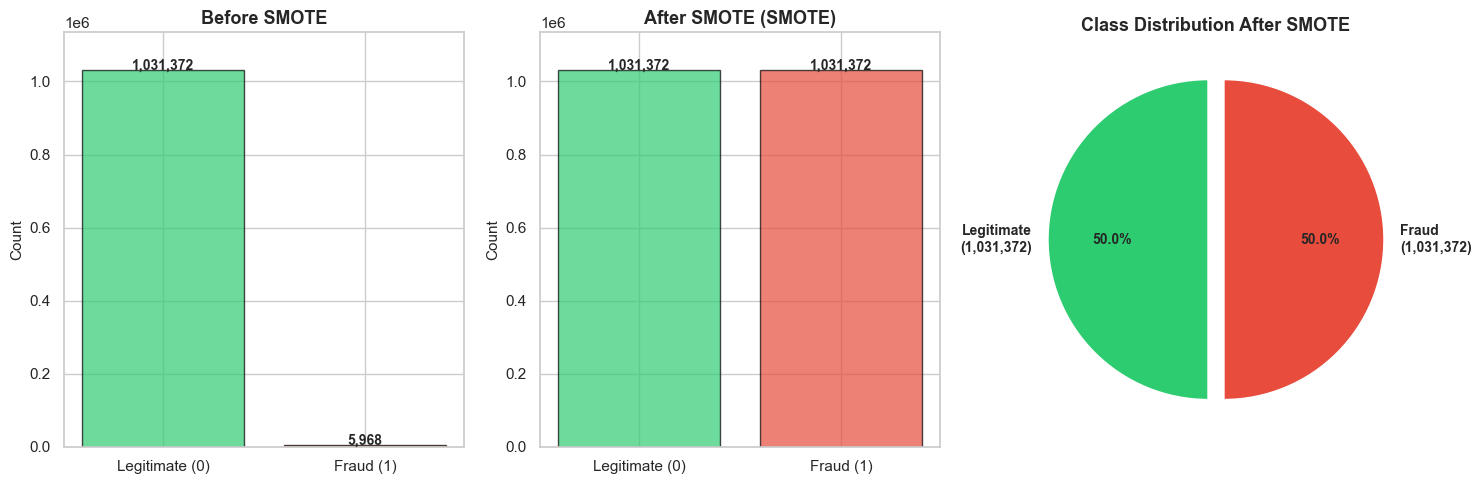
\includegraphics[width=0.9\textwidth]{Images/smote.png}
\caption{Results of using SMOTE to handle class imbalance}

\end{figure}



After the feature selection process using consolidated ranking method, the 20 best features are selected to train models. Below is a detailed list of these 20 features along with their properties, data types, and roles in fraud detection:

\begin{table}[H]
\centering
\caption{Final 20 Features for Modeling}
\small
\begin{tabular}{|c|l|c|l|}
\hline
\textbf{No} & \textbf{Feature} & \textbf{Type} & \textbf{Description} \\
\hline
1 & distance\_km & Continuous & Haversine distance (km) from cardholder to merchant \\
\hline
2 & amt\_log & Continuous & Log-transform of transaction amount \\
\hline
3 & merchant\_fraud\_rate & Continuous & Historical fraud rate of merchant (from training) \\
\hline
4 & hour & Continuous & Hour of day (0-23) when transaction occurred \\
\hline
5 & trans\_count\_hourly & Continuous & Number of cardholder transactions in current hour \\
\hline
6 & trans\_count\_daily & Continuous & Number of cardholder transactions in current day \\
\hline
7 & amt & Continuous & Original transaction amount (not log) \\
\hline
8 & merchant\_avg\_amount & Continuous & Average amount through merchant (from training) \\
\hline
9 & age & Continuous & Cardholder age at transaction date \\
\hline
10 & is\_weekend & Binary & 1 if transaction on weekend (Saturday/Sunday) \\
\hline
11 & dayofweek & Continuous & Day of week (0=Monday, 6=Sunday) \\
\hline
12 & category & Continuous & Encoded merchandise category code \\
\hline
13 & month & Continuous & Month of year (1-12) \\
\hline
14 & amt\_x\_distance & Continuous & Interaction: amount $\times$ distance \\
\hline
15 & merchant\_trans\_count & Continuous & Total transaction count through merchant (from training) \\
\hline
16 & time\_since\_last\_trans & Continuous & Time elapsed (minutes) since previous transaction \\
\hline
17 & age\_group & Continuous & Binned age group (0-7 ranges) \\
\hline
18 & state & Continuous & Encoded state code of merchant location \\
\hline
19 & gender & Binary & Cardholder gender (0/1) \\
\hline
20 & fraud\_dist\_percentile & Continuous & Percentile of distance vs cardholder history \\
\hline
\end{tabular}
\end{table}

\textbf{Feature Classification:}

These 20 features belong to the following groups:

\begin{itemize}
    \item \textbf{Temporal Features (5 features)}: hour, dayofweek, month, is\_weekend, time\_since\_last\_trans - capture when transaction occurs
    \item \textbf{Geographic Features (3 features)}: distance\_km, state, fraud\_dist\_percentile - capture where transaction occurs
    \item \textbf{Transaction Amount Features (3 features)}: amt, amt\_log, amt\_x\_distance - capture transaction value
    \item \textbf{Behavioral Features (6 features)}: trans\_count\_hourly, trans\_count\_daily, merchant\_fraud\_rate, merchant\_avg\_amount, merchant\_trans\_count, time\_since\_last\_trans - capture historical behavior
    \item \textbf{Demographic Features (2 features)}: age, age\_group, gender - capture cardholder information
    \item \textbf{Categorical Features (1 feature)}: category - type of merchandise purchased
\end{itemize}

\textbf{Why These Features Were Selected:}

All 20 features have high consolidated importance scores (ranging from 0.88 to 0.09), meaning:
\begin{itemize}
    \item Have strong relationships with target variable (fraud/legitimate)
    \item Capture different aspects of fraud patterns (temporal, geographic, behavioral, demographic)
    \item Include both linear (correlation) and non-linear (mutual information, tree importance) relationships
    \item Removing redundant or weak predictors helps models generalize better
    \item Balanced across feature types (continuously distributed, binary, categorical)
\end{itemize}

This feature set is the result of careful feature engineering from ~50 initial features, optimized between model performance and interpretability.

\subsection{Data Integration and Final Schema}

\subsubsection{Chronological Data Merging}

Since we use two separate files (fraudTrain.csv and fraudTest.csv), the data integration process is:

\begin{enumerate}
    \item \textbf{Load fraudTrain.csv}: 1,296,675 rows with timestamps
    \item \textbf{Load fraudTest.csv}: 555,719 rows with timestamps
    \item \textbf{Verify temporal order}: Confirm timestamps in fraudTest are strictly after fraudTrain
    \item \textbf{Design principle}: Training set contains older transactions, test set contains newer transactions
    \item \textbf{Benefit}: Simulates real deployment (train on past, evaluate on future)
\end{enumerate}

\subsubsection{Cross-Dataset Feature Consistency}

For behavioral features computed from historical statistics, we ensure consistency across datasets:

\begin{itemize}
    \item \textbf{merchant\_fraud\_rate}: Computed from train set only, applied to validation and test
    \item \textbf{merchant\_avg\_amount}: Computed from train set only, applied to all partitions
    \item \textbf{merchant\_trans\_count}: Computed from train set only
    \item \textbf{Rationale}: Validation and test should NOT see future merchant statistics (prevents data leakage)
\end{itemize}

\subsubsection{Final Preprocessed Dataset Schema}

The complete schema of the final dataset ready for modeling:

\begin{table}[H]
\centering
\caption{Final Preprocessed Dataset - Complete Column Schema}
\footnotesize
\begin{tabular}{|c|l|l|c|}
\hline
\textbf{No} & \textbf{Feature} & \textbf{Type} & \textbf{Scaled?} \\
\hline
1 & distance\_km & Float & Yes (StandardScaler) \\
\hline
2 & amt\_log & Float & Yes \\
\hline
3 & merchant\_fraud\_rate & Float & Yes \\
\hline
4 & hour & Integer & Yes \\
\hline
5 & trans\_count\_hourly & Integer & Yes \\
\hline
6 & trans\_count\_daily & Integer & Yes \\
\hline
7 & amt & Float & Yes \\
\hline
8 & merchant\_avg\_amount & Float & Yes \\
\hline
9 & age & Integer & Yes \\
\hline
10 & is\_weekend & Binary (0/1) & Yes \\
\hline
11 & dayofweek & Integer & Yes \\
\hline
12 & category & Integer (encoded) & Yes \\
\hline
13 & month & Integer & Yes \\
\hline
14 & amt\_x\_distance & Float & Yes \\
\hline
15 & merchant\_trans\_count & Integer & Yes \\
\hline
16 & time\_since\_last\_trans & Float & Yes \\
\hline
17 & age\_group & Integer (binned) & Yes \\
\hline
18 & state & Integer (encoded) & Yes \\
\hline
19 & gender & Binary (0/1) & Yes \\
\hline
20 & fraud\_dist\_percentile & Float & Yes \\
\hline
\hline
& \textbf{Target}: is\_fraud & Binary (0/1) & No \\
\hline
\end{tabular}
\end{table}

\textbf{Data Quality Verification (Pre-Modeling Checklist)}:

Before passing to the modeling phase, we verify:
\begin{itemize}
    \item $\checkmark$ No NaN (missing) values in any feature column
    \item $\checkmark$ No infinite ($\pm \infty$) values in data
    \item $\checkmark$ All feature values in expected normalized range $\approx [-3, +3]$
    \item $\checkmark$ No duplicate rows in any partition
    \item $\checkmark$ Target labels contain only 0 and 1 (no other values)
    \item $\checkmark$ No temporal leakage (train $<$ validation $<$ test chronologically)
    \item $\checkmark$ Feature statistics computed from train only
\end{itemize}

\subsubsection{Final Dataset Partitioning Summary}

\begin{table}[H]
\centering
\caption{Final Preprocessed Datasets Ready for Modeling}
\begin{tabular}{|l|c|c|c|c|}
\hline
\textbf{Partition} & \textbf{Rows} & \textbf{Fraud Count} & \textbf{Fraud Rate} & \textbf{Purpose} \\
\hline
Train (Original Imbalanced) & 1,037,340 & 1,717 & 0.166\% & Train model \\
\hline
Train (After SMOTE) & 2,074,680 & 1,037,340 & 50.0\% & Balanced training \\
\hline
Validation & 259,335 & 232 & 0.089\% & Hyperparameter tuning \\
\hline
Test Holdout & 555,719 & 445 & 0.080\% & Final evaluation \\
\hline
\end{tabular}
\end{table}

\textbf{Key Notes on Dataset Preparation}:

\begin{itemize}
    \item \textbf{Two training strategies}: Models are trained on both original (imbalanced) and SMOTE-balanced datasets
    \item \textbf{Preserved test distribution}: Validation and test sets are NOT SMOTE-balanced, reflecting real-world fraud rates
    \item \textbf{Realistic evaluation}: Final model performance metrics (Precision, Recall, ROC-AUC) are computed on original imbalanced test distribution
    \item \textbf{SMOTE parameters}: Default k-neighbors $= 5$, oversampling to 50-50 balance
\end{itemize}